\documentclass[12pt,a4paper]{book}
\usepackage[utf8]{inputenc}
\usepackage[T1]{fontenc}
\usepackage{amsmath}
\usepackage{amssymb}
\usepackage{ntheorem}
\usepackage[left=2.54cm, right=2.54cm, top=2.54cm, bottom=2.54cm]{geometry}
\usepackage{graphicx,svg,calc}
\graphicspath{{./fig/}}
\usepackage{ct_cmd}
\usepackage{tcolorbox}
\tcbuselibrary{breakable}
\usepackage[hidelinks]{hyperref} %for reference automatically
\usepackage{fancyhdr}
\usepackage{tikz}
\usetikzlibrary{positioning}

\begin{document}
	\title{My Lecture Note}
	\author{Phayuth}
	\maketitle
	
	\tableofcontents

	\chapter{Transfer Function}
Transfer Function is the ratio of Laplace Transform of Output of the system to the Laplace Transform of Input of the system, when all the initial condition are assumed to be zero. (Very important that if it is not zero then the system is not Linear Time Invariant)(We can not take a Laplace Transform of a nonlinear system).
Let:
\begin{itemize}
	\item {\makebox[1cm]{\(x(t)\)\hfill} is Input of the system}
	\item {\makebox[1cm]{\(y(t)\)\hfill} is Output of the system}
	\item {\makebox[1cm]{\(h(t)\)\hfill} is the system}
\end{itemize}
We have:
\begin{equation}
	y(t) = x(t)*h(t)
\end{equation}
Taking Laplace Transform, We get:
\begin{equation}
	Y(s) = X(s)*H(s)
\end{equation}
By convolution property:
\begin{equation}
	\boxed{H(s) = \frac{Y(s)}{X(s)}}
\end{equation}

\section{Example of Determine a Transfer Function}
\paragraph{System 1} Determine a Transfer Function of a system below:
\[\frac{d^2y(t)}{d t^2} + 3\frac{dy(t)}{d t} + 2 y(t) = x(t)\]
\paragraph{Solution} We have:
\begin{itemize}
	\item {\makebox[1cm]{\(x(t)\)\hfill} is Input of the system}
	\item {\makebox[1cm]{\(y(t)\)\hfill} is Output of the system}
\end{itemize}
Taking Laplace Transform of the system:
\[\mathcal{L}[\frac{d^2y(t)}{d t^2} + 3\frac{dy(t)}{d t} + 2 y(t)] = \mathcal{L}[x(t)]\]
We get:
\[\mathcal{L}[\frac{d^2y(t)}{d t^2}] = s^2Y(s) - sY(0^-) -y'(0^-)\]
\[\mathcal{L}[3\frac{dy(t)}{d t}] = 3[sY(s) - y(0)]\]
\[\mathcal{L}[2 y(t)] = 2Y(s)\]
\[\mathcal{L}[X(t)] = X(s)\]
\[s^2Y(s) - sY(0^-) -y'(0^-) + 3[sY(s) - y(0)] + 2Y(s) = X(s)\]
Put Initial Condition to zero, we get:
\[s^2Y(s) + 3sY(s) + 2Y(s) = X(s)\]
\[Y(s)[s^2 + 3s +2 ] = X(s)\]
\[\rightarrow \frac{Y(s)}{X(s)} = \frac{1}{s^2 + 3s +2}\]
\[\rightarrow H(s) = \frac{1}{s^2 + 3s +2}\]
\[\rightarrow \boxed{H(s) = \frac{1}{(s+1)(s+2)}}\]


\paragraph{System 2} Determine a Transfer Function of a system below:
\[\dot{\phi}(t) = k(\phi_{ref}(t) - \phi(t))\]
\paragraph{Solution}
\[\frac{1}{k}\dot{\phi}(t) = \phi_{ref}(t) - \phi(t)\]
\[\frac{1}{k}\dot{\phi}(t) + \phi(t) = \phi_{ref}(t)\]
Taking Laplace Transform of the system:
\[\mathcal{L}[\frac{1}{k}\dot{\phi}(t) + \phi(t)] = \mathcal{L}[\phi_{ref}(t)]\]
We have:
\begin{itemize}
	\item {\makebox[1.5cm]{\(\phi_{ref}(t)\)\hfill} is Input of the system}
	\item {\makebox[1.5cm]{\(\phi(t)\)\hfill} is Output of the system}
\end{itemize}
\[\frac{1}{k}sY(s) + Y(s) = X(s)\]
\[Y(s)[\frac{1}{k}s +1] = X(s)\]
\[\rightarrow \frac{Y(s)}{X(s)} = \frac{1}{\frac{1}{k}s + 1}\]
\[\rightarrow \boxed{H(s) = \frac{1}{\frac{1}{k}s + 1}}\]



\paragraph{System 3} Determine a Transfer Function of a system below:
\[\ddot{\phi}(t) = k(\phi_{ref}(t) - \phi(t))\]
\paragraph{Solution}
\[\frac{1}{k}\ddot{y}(t) + y(t) = x(t)\]
Taking Laplace Transform of the system:
\[\mathcal{L}[\frac{1}{k}\ddot{y}(t) + y(t)] = \mathcal{L}[x(t)]\]
\[\frac{1}{k}s^2Y(s) + Y(s) = X(s)\]
\[Y(s)[\frac{1}{k}s^2 + 1] = X(s)\]
\[\rightarrow \boxed{H(s) = \frac{1}{\frac{1}{k}s^2 + 1}}\]


\paragraph{System 4} Determine a Transfer Function of a system below:
\[\ddot{y}(t) + ky(t)= kx(t)\]
\paragraph{Solution}
Taking Laplace Transform of the system:
\[s^2Y(s) + kY(s) = kX(s)\]
\[Y(s)[s^2 + k] = kX(s)\]
\[\rightarrow \boxed{H(s) = \frac{k}{s^2 + k}}\]


\section{Example of Determine System from TF}
Below is a system transfer function that transfer wheel position $\theta$ to wheel velocity $\dot{\theta}$. Determine the system function and discretize it.
We have a TF:
\[\frac{Y(s)}{X(s)} = \frac{s}{as + 1}\]
\[(as + 1)Y(s) = sX(s)\]
\[asY(s) + Y(s) = sX(s)\]
Taking a Reverse Laplace Transform:
\[a\dot{y}(t) + y(t) = \dot{x}(t)\]
\[\rightarrow \boxed{\dot{y}(t) = -\frac{1}{a}y(t) + \frac{1}{a}\dot{x}(t)}\]
Discretize the model:
\[\frac{y_{k+1}- y_k}{T_s} = -\frac{1}{a}y_k + \frac{1}{a}\frac{x_{k+1}- x_k}{T_s}\]
\[y_{k+1}- y_k = -\frac{T_s}{a}y_k + \frac{1}{a}(x_{k+1}- x_k)\]
\[y_{k+1} = y_k - \frac{T_s}{a}y_k + \frac{1}{a}(x_{k+1}- x_k)\]
\[y_{k+1} = (1- \frac{T_s}{a})y_k + \frac{1}{a}(x_{k+1}- x_k)\]
\[\rightarrow \boxed{\dot{\theta}_{k+1} = (1- \frac{T_s}{a})\dot{\theta}_k + \frac{1}{a}(\theta_{k+1}- \theta_k)}\]
	\chapter{1st Order Differential Equation}
Differential equation is set an equation that its solution is a function and involve of its derivative. In engineering, these equations is usually used to govern a dynamics system model and the rate of change of state. In 1st Order Differential Equation is equation consist of first derivative of function in form:
\[
\frac{dy}{dx} + P(x)y = Q(x)
\]
Where :
\begin{itemize}
	\item {\makebox[1cm]{\(P(x)\)\hfill} is function of x}
	\item {\makebox[1cm]{\(Q(x)\)\hfill} is function of x}
\end{itemize}

\section{Method of Solving 1st Order Homogeneous Differential Equation}
\subsection{Method of Separation of Variable}
\begin{tcolorbox}[title=Method]
	\paragraph{When to use the Method}
	All ${y,dy}$ term and ${x,dx}$ can explicitly move to different side of the equation. For example:
	\[
	\frac{dy}{dx} = 5xy
	\]
	\[
	\rightarrow \frac{dy}{y} = 5xdx
	\]
	\paragraph{How to use the Method}
	\begin{itemize}
		\item Step 1 : Move all ${y,dy}$ term and ${x,dx}$ to different side of the equation.
		\item Step 2 : Integrate both side with respect to $ dx $ and $ dy $ respectively.
		\item Step 3 : Simplify the equation.
	\end{itemize}
\end{tcolorbox}

\paragraph{Example} Solve:
\[
\frac{dy}{dx} = 5xy
\]
\begin{itemize}
	\item Step 1
\end{itemize}
\[
\frac{dy}{y} = 5xdx
\]
\begin{itemize}
	\item Step 2
\end{itemize}
\[
\begin{split}
	\int \frac{1}{y} \,dy &= 5 \int x \,dx \\
	ln|y| &= \frac{5}{2} x^2 + c
\end{split}
\]
\begin{itemize}
	\item Step 3
\end{itemize}
\[
\begin{split}
	ln|y| &= \frac{5}{2} x^2 + c \\
	e^{ln|y|} &= e^{\frac{5}{2} x^2 + c}\\
	y &= e^{\frac{5}{2} x^2 + c}\\
	y &= e^{\frac{5}{2} x^2}e^{c}\\
	y &= Ce^{\frac{5}{2} x^2} \leftarrow Solution\\ 
\end{split}
\]


\section{Method of Solving 1st Order Non-Homogeneous Differential Equation}
\subsection{Method of Variable Substitution}
\begin{tcolorbox}[title=Method]
	\paragraph{When to use the Method} Use in general form of 1st order linear differential equation of:
	\[\frac{dy}{dx} + P(x)y = Q(x)\]
	\paragraph{How to use the Method}
	\begin{itemize}
		\item Step 1 : Substitute $ y = uv $ and $ \frac{dy}{dx} = u\frac{dv}{dx} + v \frac{du}{dx}$ to equation.
		\item Step 2 : Factoring $ v $ out. example: $ v(term\_u, term\_x) $.
		\item Step 3 : Put $ v $ term equal to zero and solve for $ u $ using separation of variable.
		\item Step 4 : Substitute $ u $ back to equation Step 2 where $ v $ term is zero and Solve for $ v $.
		\item Step 5 : After getting $ u $ and $v$, substitute back into $ y = uv $ for a solution of function.
	\end{itemize}
\end{tcolorbox}

\paragraph{Example} Solve:
\[
\frac{dy}{dx} - \frac{y}{x}= 1
\]
\begin{itemize}
	\item Step 1
\end{itemize}
\[
u\frac{dv}{dx} + v \frac{du}{dx} - \frac{uv}{x}= 1
\]
\begin{itemize}
	\item Step 2
\end{itemize}
\[
u\frac{dv}{dx} + v( \frac{du}{dx} - \frac{u}{x})= 1
\]
\begin{itemize}
	\item Step 3
\end{itemize}
\[
\begin{split}
	( \frac{du}{dx} - \frac{u}{x}) &= 0  \\
	\frac{du}{dx} &= \frac{u}{x} \\
	\frac{du}{u} &= \frac{dx}{x} \\
	\int \frac{du}{u} &= \int \frac{dx}{x} \\
	ln|u| &= ln|x| + C \\
	ln|u| &= ln|x| + ln|K| \leftarrow \text{let C = ln|k| make easier} \\
	u &= Kx
\end{split}
\]
\begin{itemize}
	\item Step 4
\end{itemize}
\[
\begin{split}
	Kx\frac{dv}{dx} &= 1 \\
	dv &= \frac{1}{Kx} dx \\
	\int dv &= \frac{1}{K}\int \frac{1}{x} dx \\
	v &= \frac{1}{K} (ln|x| + D) \\
	v &= \frac{1}{K} ln|Lx|
\end{split}
\]
\begin{itemize}
	\item Step 5
\end{itemize}
Our Solution is:
\[
y = uv = Kx\frac{1}{K} ln|Lx| = xln|Lx|
\]


\subsection{Method of Integrating Factor}
\begin{tcolorbox}[title=Method]
	Use in general form of 1st order linear differential equation of:
	\[\frac{dy}{dx} + P(x)y = Q(x)\]
	\paragraph{How to use the Method}
	\begin{itemize}
		\item Step 1 : Calculate Integrating Factor $ I(x) = e^{\int P(x)dx}$.
		\item Step 2 : Multiply both side of the equation by $ I(x) $
		\item Step 3 : Form $ \frac{d}{dx} (y.I(x)) = I(x)Q(x)$ and Integrate both side by $ dx $.
		\item Step 4 : Solve for $ y $ and simplify.
	\end{itemize}
\end{tcolorbox}

\paragraph{Example} Solve:
\[
cos(x)\frac{dy}{dx} + sin(x)y= 1
\]
Then :
\[
\frac{dy}{dx} + tan(x)y= \frac{1}{cos(x)}
\]
We have $ P(x) = tan(x)$ and $ Q(x) = \frac{1}{cos(x)} $
\begin{itemize}
	\item Step 1
\end{itemize}
\[
I(x) = e^{\int P(x)dx} = e^{\int tan(x)dx} = e^{ln|sec(x)|} = sec(x)
\]
\begin{itemize}
	\item Step 2
\end{itemize}
\[
sec(x)\frac{dy}{dx} + sec(x)tan(x)y= sec(x)\frac{1}{cos(x)}
\]
\[
sec(x)\frac{dy}{dx} + sec(x)tan(x)y= sec^2(x)
\]
\begin{itemize}
	\item Step 3
\end{itemize}
\[
\begin{split}
	\frac{d}{dx}(y.sec(x)) &= sec^2(x) \\
	\int \frac{d}{dx}(y.sec(x))dx &= \int sec^2(x) dx\\
	y.sec(x) &= \int sec^2(x) dx\\
	y.sec(x) &= tan(x) + C\\
\end{split}
\]
\begin{itemize}
	\item Step 4
\end{itemize}
\[
\begin{split}
	y.sec(x) &= tan(x) + C\\
	y &= \frac{tan(x) + C}{sec(x)} \\
	y &= sin(x) + Ccos(x)
\end{split}
\]
	\chapter{2nd Order Differential Equation}
Differential equation is set an equation that its solution is a function and involve of its derivative. In engineering, these equations is usually used to govern a dynamics system model and the rate of change of state. In 2nd Order Differential Equation is equation consist of second and first derivative of function in form:
\[
\frac{d^2y}{dx^2} + P(x)\frac{dy}{dx} + Q(x) y = f(x)
\]
\section{Method of Solving 2nd Order Homogeneous Differential Equation}
The 2nd Order Homogeneous Differential Equation has the form of:
\[
\frac{d^2y}{dx^2} + P(x)\frac{dy}{dx} + Q(x) y = 0
\]
\subsection{Method of Using Characteristic Equation}
\begin{tcolorbox}[title=Method,breakable]
	\paragraph{Where Does it come from ?}
	We propose a solution the 2nd Order Homogeneous Differential Equation above where:
	\[
	y = e^{rx}
	\]
	Thus
	\[
	\frac{d^2y}{dx^2}= r^2e^{rx}
	\]
	\[
	\frac{dy}{dx} = re^{rx}
	\]
	Substitute to the equation:
	\[
	\begin{split}
		r^2e^{rx} + P(x)re^{rx} + Q(x)e^{rx} &= 0 \\
		e^{rx} (r^2 + P(x)r + Q(x)) &= 0 \\
	\end{split}
	\]
	The term $e^{rx}$ can not go to zero, thus the term $r^2 + P(x)r + Q(x)$ will go to zero. The term $r^2 + P(x)r + Q(x)$ is the second order polynomial equation where we have three different form of solution.
	\begin{itemize}
		\item {\makebox[1cm]{\(\Delta > 0\)\hfill} the equation has 2 distinct real roots \(r_1\) and \(r_2\)}
		\item {\makebox[1cm]{\(\Delta = 0\)\hfill} the equation has repeated real root \(r\)}
		\item {\makebox[1cm]{\(\Delta < 0\)\hfill} the equation has 2 complex conjugated roots \(r_1 = \alpha + \beta i\) and \(r_2 = \alpha - \beta i\)}
	\end{itemize}
	If:
	\begin{itemize}
		\item {\makebox[1cm]{\(\Delta > 0\)\hfill} the solution has a form of \(y = Ae^{r_1x} + Be^{r_2x}\)}
		\item {\makebox[1cm]{\(\Delta = 0\)\hfill} the solution has a form of \(y = Ae^{rx} + Bxe^{rx}\)}
		\item {\makebox[1cm]{\(\Delta < 0\)\hfill} the solution has a form of}
		\begin{itemize}
			\item \(y = Ae^{(\alpha + \beta i)x} + Be^{(\alpha - \beta i)x}\)
			\item \(y = e^{\alpha x}(Ae^{\beta ix} + Be^{-\beta ix})\)
			\item \(y = e^{\alpha x}(A cos (\beta x) + iB sin (\beta x))\) (From euler's formula \(e^{ix} = cos(x)+isin(x)\))
		\end{itemize}
	\end{itemize}
	\paragraph{How to use it}
	\begin{itemize}
		\item Step 1 : Form a Characteristic Equation from the equation \(ar^2 + br + c =0\).
		\item Step 2 : Find \(\Delta\) and roots of the equation.
		\item Step 3 : Plug the result into three of the solution form and determine the constants using initial condition.
	\end{itemize}
\end{tcolorbox}

\paragraph{Example 1} Solve:
\[
\frac{d^2y}{dx^2} -9\frac{dy}{dx} + 20 y = 0
\]
\begin{itemize}
	\item Step 1
\end{itemize}
\[
r^2 -9r + 20 =0
\]
\begin{itemize}
	\item Step 2
\end{itemize}
\[
\Delta > 0, r_1 = 4, r_2 = 5
\]
\begin{itemize}
	\item Step 3
\end{itemize}
\[
y = Ae^{4x} + Be^{5x}
\]

\paragraph{Example 2} Solve:
\[
\frac{d^2y}{dx^2} -10\frac{dy}{dx} + 25 y = 0
\]
\begin{itemize}
	\item Step 1
\end{itemize}
\[
r^2 -10r + 25 =0
\]
\begin{itemize}
	\item Step 2
\end{itemize}
\[
\Delta = 0, r = 5
\]
\begin{itemize}
	\item Step 3
\end{itemize}
\[
y = Ae^{5x} + Bxe^{5x}
\]


\paragraph{Example 3} Solve:
\[
\frac{d^2y}{dx^2} -4\frac{dy}{dx} + 13 y = 0
\]
\begin{itemize}
	\item Step 1
\end{itemize}
\[
r^2 -4r + 13 =0
\]
\begin{itemize}
	\item Step 2
\end{itemize}
\[
\Delta < 0, r_1 = 2+3i, r_2 = 2-3i
\]
\begin{itemize}
	\item Step 3
\end{itemize}
\[
y = e^{2 x}(A cos (3 x) + iB sin (3 x))
\]




\section{Method of Solving 2nd Order Non-Homogeneous Differential Equation}
The 2nd Order Non-Homogeneous Differential Equation has the form of:
\[
\frac{d^2y}{dx^2} + P(x)\frac{dy}{dx} + Q(x) y = f(x)
\]
The solution of the 2nd Order Non-Homogeneous Differential Equation has a combination of General solution and Particular solution \(y = y_h + y_p\). The General solution is found by finding the solution of the equation in its homogeneous form while the Particular solution is found by finding the solution of the equation in its non-homogeneous.

\subsection{Method of Undetermined Coefficients}
\begin{tcolorbox}[title=Method]
	\paragraph{How to use it}
	\begin{itemize}
		\item Step 1 : Find \(y_h\) from the equation in homogeneous form.
		\item Step 2 : Propose \(y_p\) by guessing the form of solution from the non-homogeneous term. Use the table for help. And determine the constants of the \(y_p\).
		\item Step 3 : Find \(y = y_h + y_p\) and Find remaining constants from initial equation.
	\end{itemize}
	\textbf{Table of solution form}
	\begin{tabular}{|c|c|}
		\hline
		\(f(x)\)         & \(y_p\)                                 \\
		\hline
		1                & \(a\)                                   \\
		\hline
		\(5x+7\)         & \(ax+b\)                                \\
		\hline
		\(3x^2-2\)       & \(ax^2+b+c\)                            \\
		\hline
		\(x^3-x+1\)      & \(ax^3+bx^2+cx+d\)                      \\
		\hline
		\(sin4x\)        & \(acos4x+bsin4x\)                       \\
		\hline
		\(cos4x\)        & \(acos4x+bsin4x\)                       \\
		\hline
		\(e^{5x}\)       & \(ae^{5x}\)                             \\
		\hline
		\((9x-2)e^{5x}\) & \((ax+b)e^{5x}\)                        \\
		\hline
		\(x^2e^{5x}\)    & \((ax^2+b+c)e^{5x}\)                    \\
		\hline
		\(e^{3x}sin4x\)  & \(ae^{3x}cos4x+be^{3x}sin4x\)           \\
		\hline
		\(5x^2sin4x\)    & \((ax^2+b+c)cos4x+(dx^2+e+f)sin4x\)     \\
		\hline
		\(xe^{3x}cos4x\) & \((ax+b)e^{3x}cos4x+(cx+d)e^{3x}sin4x\) \\
		\hline
	\end{tabular}
\end{tcolorbox}


\paragraph{Example} Solve:
\[
\frac{d^2y}{dx^2} - y= 2x^2 - x - 3
\]
\begin{itemize}
	\item Step 1
\end{itemize}
\[
\begin{split}
	r^2 - 1 &= 0 \\
	\Delta > 0 &, r_1=1,r_2=-1 \\
	y_h &= Ae^{1x} + Be^{-1x}
\end{split}
\]
\begin{itemize}
	\item Step 2
\end{itemize}
Let guess the form based on the \(2x^2 - x - 3\), because of it is a polynomial let guess \(y_p = ax^2 + bx + c\)
\[
\begin{split}
	\frac{dy_p}{dx} &= 2ax+b \\
	\frac{d^2y_p}{dx^2} &= 2a \\
\end{split}
\]
Substitute back to equation
\[
\begin{split}
	2a - (ax^2 + bx + c) &= 2x^2 - x - 3 \\
	2a - ax^2 - bx - c &= 2x^2 - x - 3 \\
	-ax^2-bx+2a-c &=2x^2 - x - 3 \\
	-a &= 2 \\
	-b &= -1 \\
	2a-c &= -3 \\
	\rightarrow a &= -2 \\
	\rightarrow b &= 1 \\
	\rightarrow c &= -1 \\
\end{split}
\]
Thus
\[
y_p = -2x^2 + x - 1
\]
\begin{itemize}
	\item Step 3
\end{itemize}
\[
y =  Ae^{1x} + Be^{-1x} -2x^2 + x - 1
\]
	\chapter{2nd Order ODE Standard Form}
This section, we study on system of 2nd Order ODE with Standard Form Natural Frequency and Damping Ratio.
\section{Spring Mass Damper Modeling}
(Free Body Diagram)

\[
\begin{split}
	-kx(t) - b\dot{x}(t) &= m\ddot{x}(t) \\
	m\ddot{x}(t) + kx(t) + b\dot{x}(t)&= 0 \\
	\ddot{x} + \frac{b}{m} \dot{x}+\frac{k}{m} x(t) &= 0
\end{split}
\]
Let have the differential model above to look like the General Standard Form of :
\[
\boxed{\ddot{x}(t)+2\zeta\omega_n\dot{x}(t)+\omega_n^2x(t)=0}
\]
Where :
\begin{itemize}
	\item $ \zeta $ is damping ratio
	\item $ \omega_n $ is natural frequency
\end{itemize}
Thus, we have :
\begin{itemize}
	\item $ \frac{b}{m} = 2\zeta\omega_n \rightarrow \zeta = \frac{b}{2\sqrt{km}}$ 
	\item $ \frac{k}{m} = \omega_n^2 \rightarrow \omega_n = \sqrt{\frac{k}{m}}$
\end{itemize}
Let solve the Standard Form $ x(t) $:
\[ 
\ddot{x}(t)+2\zeta\omega_n\dot{x}(t)+\omega_n^2x(t)=0 
\]
Using Laplace Transform :
\[ 
\begin{split}
	s^2 X(s) - sx(0) -  \dot{x}(0) + 2\zeta\omega_n(sX(s)-x(0)) + \omega_n^2X(s) = 0 \\
	s^2 X(s) - sx_0 -  \dot{x}_0 + 2\zeta\omega_n(sX(s)-x_0) + \omega_n^2X(s) = 0 \\
\end{split}
\]
\[ 
X(s) = \frac{sx_0 + \dot{x}_0 + 2\zeta\omega_nx_0}{s^2 + 2\zeta\omega_ns+\omega_n^2}
\]
Let Find the root of the Denominator of $ X(s) $. From solving the 2nd order quadratic formula, we have the root :
\[ 
s_{1,2} = \frac{-2\zeta\omega_n \pm \sqrt{(2\zeta\omega_n)^2 - 4\omega_n^2}}{2} = -\zeta\omega_n \pm \omega_n\sqrt{\zeta^2-1}
\]
From the root, we can see that there are 3 cases:
\begin{itemize}
	\item Distinct Real Root
	\item Double Real Root
	\item Complex Root
\end{itemize}


\subsection{Distinct Real Roots}
To have the Distinct Real Root Case, We need:
\[ 
\begin{split}
	(2\zeta\omega_n)^2 - 4\omega_n^2 &> 0 \\
	4\zeta^2\omega_n^2 - 4\omega_n^2 &> 0 \\
	4\omega_n^2 (\zeta^2 - 1) &> 0 \\
	(\zeta^2 - 1) &> 0 \\
	\zeta^2  &> 1 \\
	\zeta &> 1
\end{split}
\]
We get Over-damped Case from the damping ratio of $ \boxed{\zeta > 1} $


\subsection{Double Real Root}
To have the Double Real Root Case, We need:
\[ 
\begin{split}
	(2\zeta\omega_n)^2 - 4\omega_n^2 &= 0 \\
	4\zeta^2\omega_n^2 - 4\omega_n^2 &= 0 \\
	4\omega_n^2 (\zeta^2 - 1) &= 0 \\
	(\zeta^2 - 1) &= 0 \\
	\zeta^2  &= 1 \\
	\zeta &= 1
\end{split}
\]
We get Critically damped Case from the damping ratio of $ \boxed{\zeta = 1} $. From the mathematical perspective, the damping ratio is unity (1) mean Critically damped. Where some people from control perspective prefer the damping ratio of $ \frac{1}{\sqrt{2}} $ to be Critically damped.


\subsection{Complex Root}
To have the Complex Root Case, We need:
\[ 
\begin{split}
	(2\zeta\omega_n)^2 - 4\omega_n^2 &< 0 \\
	4\zeta^2\omega_n^2 - 4\omega_n^2 &< 0 \\
	4\omega_n^2 (\zeta^2 - 1) &< 0 \\
	(\zeta^2 - 1) &< 0 \\
	\zeta^2  &< 1 \\
	\zeta &< 1
\end{split}
\]

\section{Discussion of Each Cases}
\subsection{Over-damped Case ($ \zeta > 1$)}
Above equation can be written as:
\[ 
X(s) = \frac{sx_0 + \dot{x}_0 + 2\zeta\omega_nx_0}{s^2 + 2\zeta\omega_ns+\omega_n^2} = \frac{a_1}{s+r_1}+\frac{a_2}{s+r_2}
\]
After using Partial Fraction Decomposition, we get:
\[ 
a_1 = \frac{-\dot{x}_0 + x_0 (-\zeta \omega_n + \sqrt{(\zeta^2-1)\omega_n^2})}{2\sqrt{(\zeta^2-1)\omega_n^2}}
\]
\[ 
a_2 = \frac{\dot{x}_0 + x_0 (\zeta \omega_n + \sqrt{(\zeta^2-1)\omega_n^2})}{2\sqrt{(\zeta^2-1)\omega_n^2}}
\]
Thus the solution of differential equation $ \ddot{x}(t)+2\zeta\omega_n\dot{x}(t)+\omega_n^2x(t)=0  $ where $ x(0)=x_0, \dot{x}(0) = \dot{x}_0 $ is :
\[ 
x(t) = a_1e^{r_1t}+a_2e^{r_2t} 
\]
Where:
\[
\begin{split}
	a_1 &= \frac{-\dot{x}_0 + x_0 (-\zeta \omega_n + \sqrt{(\zeta^2-1)\omega_n^2})}{2\sqrt{(\zeta^2-1)\omega_n^2}} \\
	a_2 &= \frac{\dot{x}_0 + x_0 (\zeta \omega_n + \sqrt{(\zeta^2-1)\omega_n^2})}{2\sqrt{(\zeta^2-1)\omega_n^2}} \\
	r_1,r_2 &= -\zeta\omega_n \pm \omega_n\sqrt{\zeta^2-1}
\end{split} 
\]

\subsection{Critically damped Case ($ \zeta = 1$)}
We have the root : $ r_1,r_2 = -\zeta\omega_n \pm \omega_n\sqrt{\zeta^2-1} $\\
By substitute $ \zeta = 1 $, we get the root : 
\[ r_1,r_2 = -\omega_n \]
Above equation can be written as:
\[ 
X(s) = \frac{sx_0 + \dot{x}_0 + 2\zeta\omega_nx_0}{s^2 + 2\zeta\omega_ns+\omega_n^2} = \frac{a_1}{s+\omega_n}+\frac{a_2}{(s+\omega_n)^2}
\]
After using Partial Fraction Decomposition, we get:
\[ 
a_1 = x_0
\]
\[ 
a_2 = \dot{x}_0 + x_0\omega_n
\]
Thus the solution of differential equation $ \ddot{x}(t)+2\zeta\omega_n\dot{x}(t)+\omega_n^2x(t)=0  $ where $ x(0)=x_0, \dot{x}(0) = \dot{x}_0 $ is :
\[ 
x(t) = x_0e^{-\omega_nt}+te^{-\omega_nt}(\dot{x}_0+x_0\omega_n)
\]
Where:
\[
\begin{split}
	a_1 &= x_0\\
	a_2 &= \dot{x}_0 + x_0\omega_n
\end{split} 
\]


\subsection{Under damped Case ($ \zeta < 1$)}
We have the root : $ r_1,r_2 = -\zeta\omega_n \pm \omega_n\sqrt{\zeta^2-1} $\\
By modify the square root part, we get :
\[
\begin{split}
	r_1,r_2 &= -\zeta\omega_n \pm \omega_n\sqrt{-1(1-\zeta^2)} \\
	&= -\zeta\omega_n \pm \omega_n\sqrt{(1-\zeta^2)}\sqrt{-1} \\
	&= -\zeta\omega_n \pm \omega_n\sqrt{(1-\zeta^2)}i \\
\end{split}
\]
Let:
\[
\begin{split}
	\sigma &= \zeta\omega_n\\
	\omega_d &=\omega_n\sqrt{(1-\zeta^2)} \\
\end{split}
\]
We can write the root as :
\[
r_1,r_2 = -\sigma \pm \omega_d i
\]
Rewrite the root in form of :
\[
s^2 + 2\zeta\omega_ns+\omega_n^2 = (s+\alpha)^2+w_n^2
\]
We get :
\[
\begin{split}
	\alpha &= \zeta\omega_n\\
	\omega &= \sqrt{(1-\zeta^2)\omega_n^2} \\
\end{split}
\]
Above equation can be written as:
\[ 
X(s) = \frac{sx_0 + \dot{x}_0 + 2\zeta\omega_nx_0}{s^2 + 2\zeta\omega_ns+\omega_n^2} = \frac{sx_0 + \dot{x}_0 + 2\zeta\omega_nx_0}{(s+\alpha)^2+w_n^2}
\]
After using Partial Fraction Decomposition, The solution of differential equation $ \ddot{x}(t)+2\zeta\omega_n\dot{x}(t)+\omega_n^2x(t)=0  $ where $ x(0)=x_0, \dot{x}(0) = \dot{x}_0 $ is :
\[
x(t) = a cos(\omega t) + b sin(\omega t)
\]
Where:
\[
\begin{split}
	a &= x_0e^{-\alpha t}\\
	b &= \frac{\dot{x}_0 + x_0\zeta\omega_n}{\omega} e^{-\alpha t}\\
	\alpha &= \zeta\omega_n \\
	\omega &= \sqrt{(1-\zeta^2)\omega_n^2} \\
\end{split} 
\]
Or in simple form of :
\[
x(t) = A e^{-\zeta \omega_n t}cos(\omega_d t - \phi)
\]
Where:
\[
\begin{split}
	A &= \sqrt{x_0^2 + \frac{(\dot{x}_0 + x_0\zeta\omega_n)^2}{(1-\zeta^2)\omega_n^2}}\\
	\omega_d &= \omega_n\sqrt{(1-\zeta^2)} \\
	\phi & = atan2(\frac{\dot{x}_0 + x_0\zeta\omega_n}{\omega_n\sqrt{(1-\zeta^2)}},x_0)
\end{split} 
\]
	\chapter{Partial Fraction Decomposition}
Usually we have a Function:
\[
F(s) = \frac{A(s)}{B(s)}
\]
Where:
\begin{itemize}
	\item {\makebox[1cm]{\(A(s)\)\hfill} is a polynomial which order is smaller than \(B(s)\)}
	\item {\makebox[1cm]{\(B(s)\)\hfill} is a polynomial which order is greater than \(A(s)\)}
\end{itemize}
To perform the Partial Fraction Decomposition, first we have to get \(F(s)\) into the ZPK (Zero, Pole, Gain) format which is:
\[
F(s) = \frac{K (s+z_1)(s+z_2)(s+z_3)...(s+z_n)}{(s+p_1)(s+p_2)(s+p_3)...(s+p_n)}
\]
Where:
\begin{itemize}
	\item {\makebox[1cm]{\(z\)\hfill} is roots of \(A(s)\) that is the zeros of \(F(s)\)}
	\item {\makebox[1cm]{\(p\)\hfill} is roots of \(B(s)\) that is the poles of \(F(s)\)}
\end{itemize}
Given denominator of \(F(s)\), determine the pole of the polynomial \((s+p_1)...(s+p_n)\). From the result we can divide into 3 cases.
\section{Case 1: Distinct Real Poles}
\begin{tcolorbox}[title=Method]
	In this case we can propose that the \(F(s) = \frac{A(s)}{B(s)}\) can be written into:
	\[
	F(s) = \frac{a_1}{s+p_1} + \frac{a_2}{s+p_2} + ... + \frac{a_n}{s+p_n}
	\]
\end{tcolorbox}

\paragraph{Example}
\[
F(s) = \frac{s^2+8s+15}{s^3+3s^2+2s}
\]
We can see that Nominator order is greater than Denominator order. And the denominator \(s^3+3s^2+2s\) has the roots \(s_1=0 , s_2=-2 , s_3=-1 \rightarrow p_1=0, p_2=2, p_3=1\). Thus we have:
\[
F(s) = \frac{s^2+8s+15}{s^3+3s^2+2s} = \frac{s^2+8s+15}{(s+0)(s+2)(s+1)} = \frac{a_1}{s+0} + \frac{a_2}{s+2} + \frac{a_3}{s+1} 
\]
So we have to find \(a_1,a_2,a_3\) to make it work. We can use 2 methods to do it.

\paragraph{Method 1} Multiplication

\[
\frac{s^2+8s+15}{s(s+2)(s+1)} = \frac{a_1}{s} + \frac{a_2}{s+2} + \frac{a_3}{s+1} 
\]
Multiply both side in terms of \(a_1\) \((s)\):
\[
\begin{split}
	s(\frac{s^2+8s+15}{s(s+2)(s+1)}) &= s\frac{a_1}{s} + s\frac{a_2}{s+2} + s\frac{a_3}{s+1} \\
	\frac{s^2+8s+15}{(s+2)(s+1)} &= a_1 + s\frac{a_2}{s+2} + s\frac{a_3}{s+1}
\end{split}
\]
Substitute \(s=0\)
\[
\begin{split}
	\frac{0+0+15}{(0+2)(0+1)} &= a_1 + 0 + 0 \\
	a_1 &= \frac{15}{2}
\end{split}
\]
Multiply both side in terms of \(a_2\) \((s+2)\):
\[
\begin{split}
	(s+2)(\frac{s^2+8s+15}{s(s+2)(s+1)}) &= (s+2)\frac{a_1}{s} + (s+2)\frac{a_2}{s+2} + (s+2)\frac{a_3}{s+1} \\
	\frac{s^2+8s+15}{(s)(s+1)} &= (s+2)\frac{a_1}{s} + a_2 + (s+2)\frac{a_3}{s+1}
\end{split}
\]
Substitute \(s=-2\)
\[
\begin{split}
	\frac{(-2)^2+8(-2)+15}{(-2)(-2+1)} &= (-2+2)\frac{a_1}{-2} + a_2 + (-2+2)\frac{a_3}{-2+1} \\
	\frac{4-16+15}{2} &= 0 + a_2 + 0 \\
	a_2 &= \frac{3}{2}
\end{split}
\]
Multiply both side in terms of \(a_3\) \((s+1)\):
\[
\begin{split}
	(s+1)(\frac{s^2+8s+15}{s(s+2)(s+1)}) &= (s+1)\frac{a_1}{s} + (s+1)\frac{a_2}{s+2} + (s+1)\frac{a_3}{s+1} \\
	\frac{s^2+8s+15}{(s)(s+2)} &= (s+1)\frac{a_1}{s} + (s+1)\frac{a_2}{s+2} + a_3 \\
\end{split}
\]
Substitute \(s=-1\)
\[
\begin{split}
	\frac{(-1)^2+8(-1)+15}{(-1)(-1+2)} &= (-1+1)\frac{a_1}{-1} + (-1+1)\frac{a_2}{-1+2} + a_3 \\
	\frac{1+-8+15}{-1} &= 0 + 0 + a_3 \\
	a_3 &= -8
\end{split}
\]
So we get:
\[
\boxed{F(s) = \frac{s^2+8s+15}{s^3+3s^2+2s} = \frac{\frac{15}{2}}{s} + \frac{\frac{3}{2}}{s+2} + \frac{-8}{s+1}}
\]

\paragraph{Method 2} Coefficient

\[
\frac{s^2+8s+15}{s(s+2)(s+1)} = \frac{a_1}{s} + \frac{a_2}{s+2} + \frac{a_3}{s+1} 
\]
Get the right-hand side denominator the same as left-hand side.
\[
\begin{split}
	\frac{s^2+8s+15}{s(s+2)(s+1)} &= \frac{(s+1)(s+2)a_1+s(s+1)a_2+s(s+2)a_3}{s(s+2)(s+1)} \\
	s^2+8s+15 &= (s+1)(s+2)a_1+s(s+1)a_2+s(s+2)a_3 \\
	&= (s^2+2s+s+2)a_1 + (s^2+s)a_2 + (s^2+2s)a_3 \\
	&= (s^2+3s+2)a_1 + (s^2+s)a_2 + (s^2+2s)a_3 \\
	&= s^2a_1+3sa_1+2a_1 + s^2a_2+sa_2 + s^2a_3+2sa_3 \\
	s^2+8s+15 &= s^2(a_1+a_2+a_3) + s(3a_1+a_2+2a_3) + (2a_1)\\
	1 &= a_1+a_2+a_3 \\
	8 &= 3a_1+a_2+2a_3 \\
	15 &= 2a_1 \\
	a_1 &= \frac{15}{2} \\
	a_2 &= \frac{3}{2} \\
	a_3 &= -8
\end{split}
\]
So we get:
\[
\boxed{F(s) = \frac{s^2+8s+15}{s^3+3s^2+2s} = \frac{\frac{15}{2}}{s} + \frac{\frac{3}{2}}{s+2} + \frac{-8}{s+1}}
\]

\section{Case 2: Repeated Real Poles}
\begin{tcolorbox}[title=Method]
	In this case we can propose that the \(F(s) = \frac{A(s)}{B(s)}\) can be written into:
	\[
	F(s) = \frac{a_1}{s+p} + \frac{a_2}{(s+p)^2} + ... + \frac{a_n}{(s+p)^n}
	\]
\end{tcolorbox}

\paragraph{Example}
\[
F(s) = \frac{s^2+2s+3}{(s+1)^3}
\]
The denominator \((s+1)^3\) has a repeated real pole at \(p=-1\). \(F(s)\) can be written as:
\[
F(s) = \frac{s^2+2s+3}{(s+1)^3} = \frac{a_1}{s+1} + \frac{a_2}{(s+1)^2} + \frac{a_3}{(s+1)^3}
\]

\paragraph{Method 1} Coefficient

Determine \(a_1,a_2,a_3\)
\[
\begin{split}
	\frac{s^2+2s+3}{(s+1)^3} &= \frac{(s+1)^2a_1}{(s+1)^2(s+1)} + \frac{(s+1)a_2}{(s+1)(s+1)^2} + \frac{a_3}{(s+1)^3} \\
	\frac{s^2+2s+3}{(s+1)^3} &= \frac{(s+1)^2a_1+(s+1)a_2+a_3}{(s+1)^3} \\
	s^2+2s+3 &= (s+1)^2a_1+(s+1)a_2+a_3 \\
	s^2+2s+3 &= s^2 a_1 + 2s a_1 + a_1+ sa_2 + a_2 + a_3 \\
	s^2+2s+3 &= s^2 a_1 + s(2a_1+a_2) + (a_1+a_2+a_3)\\
\end{split}
\]
\[
\begin{split}
	1 &= a_1 \\
	2 &= 2a_1+a_2 \\
	3 &= a_1+a_2+a_3 \\
	\rightarrow a_1 &= 1 \\
	\rightarrow a_2 &= 0 \\
	\rightarrow a_3 &= 2
\end{split}
\]
Thus we get:
\[
\boxed{
	F(s) = \frac{s^2+2s+3}{(s+1)^3} = \frac{1}{s+1} + \frac{0}{(s+1)^2} + \frac{2}{(s+1)^3} = \frac{1}{s+1} + \frac{2}{(s+1)^3}}
\]

\paragraph{Method 2} Derivative

From finding the common denominator above:
\[
s^2+2s+3 = (s+1)^2a_1+(s+1)a_2+a_3 
\]
Substitute \(s = -1\)
\[
\begin{split}
	(-1)^2+2(-1)+3 &= (-1+1)^2a_1+(-1+1)a_2+a_3 \\
	(-1)^2+2(-1)+3 &= 0+0+a_3 \\
	a_3 &= 2
\end{split}
\]
Take derivative of \(s^2+2s+3 = (s+1)^2a_1+(s+1)a_2+a_3\) both side, we get:
\[
2s+2 = 2(s+1)a_1+a_2
\]
Substitute \(s = -1\)
\[
\begin{split}
	2(-1)+2 &= 2(-1+1)a_1+a_2 \\
	2(-1)+2 &= 0+a_2 \\
	a_2 &= 0
\end{split}
\]
Take derivative of \(2s+2 = 2(s+1)a_1+a_2\) both side, we get:
\[
\begin{split}
	2 &= 2a_1 \\
	a_1 &= 1
\end{split}
\]
Thus we get:
\[
\boxed{
	F(s) = \frac{s^2+2s+3}{(s+1)^3} = \frac{1}{s+1} + \frac{0}{(s+1)^2} + \frac{2}{(s+1)^3} = \frac{1}{s+1} + \frac{2}{(s+1)^3}}
\]



\section{Case 3: Complex Conjugate Poles}
\begin{tcolorbox}[title=Method]
In this case we can propose that the \(F(s) = \frac{A(s)}{B(s)}\) can be written into:
\[
F(s) = \frac{A(s)}{(s+\alpha)^2+\omega^2}
\]
Where from general denominator:
\[
s^2 + ds + e = 0
\]
\[
\begin{split}
	\alpha &= \frac{d}{2} \\
	\omega &= \frac{\sqrt{4e-d^2}}{2}
\end{split}
\]
\end{tcolorbox}

\paragraph{Example}
\[
F(s) = \frac{s-1}{s^2+2s+2}
\]
From denominator \(s^2+2s+2\) in general form \(d = 2, e = 2\), we get:
\[
\begin{split}
	\alpha &= 1 \\
	\omega &= 1
\end{split}
\]
Thus:
\[\boxed{
	F(s) = \frac{s-1}{s^2+2s+2} = \frac{s-1}{(s+1)^2+1^2}}
\]
\section{Improper Complex Function}
\begin{tcolorbox}[title=Method]
We have a transfer function:
\[
F(s) = \frac{A(s)}{B(s)}
\]
Where:
\begin{itemize}
	\item {\makebox[1cm]{\(A(s)\)\hfill} is a polynomial which order is greater than \(B(s)\)}
	\item {\makebox[1cm]{\(B(s)\)\hfill} is a polynomial which order is smaller than \(A(s)\)}
\end{itemize}
We can use synthetic division to make the \(A(s)\) smaller than \(B(s)\) (Polynomial Equation division).
\end{tcolorbox}
	\chapter{Laplace and Inverse Laplace Transform}
Laplace Transform convert a function in time domain into frequency domain in polynomial form. Laplace Transform is used for Analyzing and Solving Ordinary Differential Equation. By using Laplace Transform we can analyze an ODE by just analyze the polynomial equation.
\begin{tcolorbox}[title=Process]
	\begin{center}
		\textbf{Given an Ordinary Differential Equation and Initial Condition}
		\[
		a_2\ddot{x}(t) + a_1\dot{x}(t)+a_0x(t)=b_1\dot{u}(t)+b_0u(t)\quad|\quad x(0) = 0,\dot{x}(0) = 0
		\]
		\[
		\downdownarrows
		\]
		\textbf{Laplace Transform}
		\[
		X(s) = \frac{b_1s+b_0}{a_2s^2+a_1s+a_0} \frac{1}{s}
		\]
		\[
		\downdownarrows
		\]
		\textbf{Partial Fraction Decomposition}
		\[
		X(s) = \frac{k_0}{s}+\frac{k_1}{s+p_1}+\frac{k_2}{s+p_2}
		\]
		\[
		\downdownarrows
		\]
		\textbf{Inverse Laplace Transform}
		\[
		x(t) = k_0 + k_1e^{-p_1t} + k_2e^{-p_2t}
		\]
	\end{center}
\end{tcolorbox}


\section{Laplace Transform}
Definition of Laplace Transform: Given a function in time domain, its Laplace Transform is denoted by:
\[
F(s) = \mathcal{L}\{f(t)\} = \int_{0}^{\infty} f(t)e^{-st} dt
\]
Where : \(s = \sigma + j\omega\)

\subsection{Laplace of Dirac Delta Function}
We have a function :
\[
\delta(t) = \frac{1}{|a|\sqrt{\pi}}e^{-(t/a)^2}
\]
as \(a \rightarrow 0\)
\[
\Delta(s) = 1
\]

\subsection{Laplace of Unit Function}
We have a function :
\[
u(t) = 
\begin{cases}
	1, & \text{if } t\geq 0 \\
	0, & \text{if } t<0     \\
\end{cases}       
\]
We have a Laplace :
\[
U(s) = \int_{0}^{\infty} 1e^{-st} dt = -\frac{1}{s} e^{-st} |_0^\infty = -\frac{1}{s}[e^{-\infty} - e^{0}] = -\frac{1}{s}[0 - 1] = \frac{1}{s}
\]

\subsection{Laplace of $f(t) = e^{-at}$}
We have a function :
\[
f(t) = e^{-at}
\]
We have a Laplace :
\[
\begin{split}
	F(s) &= \int_{0}^{\infty} e^{-at} e^{-st} dt \\
	&= \int_{0}^{\infty} e^{-(s+a)t} dt \\
	&= -\frac{1}{s+a} \int_{0}^{\infty} (-(s+a)t)' e^{-(s+a)t} dt \\
	&= -\frac{1}{s+a} \left[e^{-(s+a)t}\right]_0^\infty  \\
	&= -\frac{1}{s+a} \left[e^{-\infty} - e^0\right]  \\
	F(s) &= \frac{1}{s+a}
\end{split}
\]

\subsection{Laplace of $f(t) = t$}
We have a function :
\[
f(t) = t
\]
We have a Laplace :
\[
F(s) = \int_{0}^{\infty} t e^{-st} dt
\]
Let :
\[
\begin{split}
	u &= t \rightarrow du = dt\\
	dv &= e^{-st} dt \rightarrow v = \int e^{-st}dt = -\frac{1}{s} e^{-st}
\end{split}
\]
\[
\begin{split}
	F(s) &= uv - \int vdu \\
	&= (t) (-\frac{1}{s} e^{-st}) - \int -\frac{1}{s} e^{-st} dt \\
	&= -\frac{t}{s} e^{-st} +\frac{1}{s} \int e^{-st} dt \\
	&= -\frac{t}{s} e^{-st} -\frac{1}{s^2} e^{-st} \\
	&= -(\frac{t}{s} +\frac{1}{s^2}) e^{-st} \\
	&= -\left((\frac{st+1}{s^2}) e^{-st} \right) |_0^\infty \\
	&= \frac{1}{s^2}
\end{split}
\]

\subsection{Laplace of Integral of a Function}
We have an integral of a function:
\[
f(t) = \int_{0}^{t} f(\tau) d\tau
\]
We have a Laplace:
\[
\begin{split}
	F(s) &= \int_{0}^{\infty} (\int_{0}^{t} f(\tau) d\tau) e^{-st} dt \\
	&= \int_{0}^{t} f(\tau) d\tau (-\frac{1}{s}) e^{-st} |_0^\infty + \int_{0}^{\infty} \frac{1}{s} e^{-st} f(t) dt \\
	&= \frac{1}{s} \int_{0}^{\infty} f(t) e^{-st} dt
\end{split}
\]

\subsection{Laplace of Derivative of a Function}
We have an integral of a function:
\[
f(t) = \frac{df(t)}{dt}
\]
We have a Laplace:
\[
\begin{split}
	F(s) &= \int_{0}^{\infty} \frac{df(t)}{dt} e^{-st} dt \\
	&= e^{-st} f(t) |_0^\infty + \int_{0}^{\infty} f(t) se^{-st} dt \\
	&= -f(0) + s \int_{0}^{\infty} f(t) e^{-st} dt
\end{split}
\]
\[
\mathcal{L}\{\frac{df(t)}{dt}\} = s\mathcal{L}\{f(t)\} - f(0)
\]


\subsection{Final Value Theorem}
FVT is used to relate the steady state behavior of \(f(t)\) to the behavior \(sF(s)\). If a function has a Laplace transform, then:
\[
\lim_{t->\infty} f(t) = \lim_{s->0} sF(s)
\]
\paragraph{Example 1} We have a system
\[
\Omega(s) = \frac{K}{s(\tau s + 1)}
\]
To find the steady state value of \(\omega(t)\), we get:
\[
\omega_{ss} = \lim_{s->0} s\frac{K}{s(\tau s + 1)} = K
\]
\paragraph{Example 2} We have a system
\[
\begin{split}
	\dot{\omega}(t) + a \omega (t) &= b u(t) \\
	s\Omega(s) + a\Omega(s) &= b U(s) \\
	\Omega(s)(s+a) &= b U(s) \\
	\Omega(s) &= \frac{b}{(s+a)} U(s)
\end{split}
\]
Case 1 : We want to study when \(u(t)=V_0\) is step function, thus \(U(s) = \frac{V_0}{s}\), we get a system:
\[
\Omega(s) = \frac{V_0b}{s(s+a)}
\]
\begin{itemize}
	\item Check if the poles of the system is on the left-half plane
\end{itemize}
By finding the roots of denominator of the system \(s\Omega(s) = \frac{sV_0b}{s(s+a)} = \frac{V_0b}{(s+a)}\). We see the root is \(s = -a\) where \(a\) is positive, thus the pole of the system in on the left-half place. \\
Finding the steady state of the system:
\[
\omega_{ss} = \lim_{s->0} s\Omega(s) = \lim_{s->0} s\frac{V_0b}{s(s+a)} = \lim_{s->0} \frac{V_0b}{(s+a)} = \frac{V_0b}{a}
\]
Case 2 : We want to study when \(u(t)=t\) is ramp function, thus \(U(s) = \frac{1}{s^2}\), we get a system:
\[
\Omega(s) = \frac{b}{s^2(s+a)}
\]
\begin{itemize}
	\item Check if the poles of the system is on the left-half plane
\end{itemize}
By finding the roots of denominator of the system \(s\Omega(s) = s\frac{b}{s^2(s+a)} = \frac{b}{s(s+a)}\). We see the root is \(s = -a\) and \(s=0\). The root \(s=0\) is exactly on the imaginary axis, thus the pole of the system in not on the left-half place. Thus the system will not come to rest at the final value.




\section{Inverse Laplace Transform}
We want to inverse the Laplace Transform from frequency domain back to time domain.
\[
f(t) = \mathcal{L}^{-1}[F(s)] = \oint_{{\gamma-iT}}^{{\gamma+iT}} e^{st} F(s) ds
\]
From the inverse Laplace Transform from definition, it is very hard. We want to manipulate the Laplace Transform into an easier and recognizable form to easily inverse it. 

\subsection{Case 1: Distinct Real Poles}
\paragraph{Example}
\[
F(s) = \frac{s^2+8s+15}{s^3+3s^2+2s} = \frac{7.5}{s} + \frac{-8}{s+1} + \frac{1.5}{s+2}
\]
\[
\begin{split}
	\mathcal{L}^{-1}[F(s)] &= \mathcal{L}^{-1}[\frac{7.5}{s}] + \mathcal{L}^{-1}[\frac{-8}{s+1}] + \mathcal{L}^{-1}[\frac{1.5}{s+2}] \\
	&= 7.5\mathcal{L}^{-1}[\frac{1}{s}] -8\mathcal{L}^{-1}[\frac{1}{s+1}] + 1.5\mathcal{L}^{-1}[\frac{1}{s+2}] \\
	f(t) &= 7.5.1(t) -8e^{-1t} + 1.5e^{-2t}
\end{split}
\]
\subsection{Case 2: Repeated Real Poles}
\paragraph{Example}
\[
F(s) = \frac{s^2+2s+3}{(s+1)^3} = \frac{1}{s+1} + \frac{2}{(s+1)^3}
\]
\[
\begin{split}
	\mathcal{L}^{-1}[F(s)] &= \mathcal{L}^{-1}[\frac{1}{s+1}] + \mathcal{L}^{-1}[\frac{2}{(s+1)^3}] \\
	&= \mathcal{L}^{-1}[\frac{1}{s+1}] + 2\mathcal{L}^{-1}[\frac{1}{(s+1)^3}] \\
	&= e^{-1t} + 2(\frac{1}{(3-1)!}t^{3-1}e^{-1t}) \\
	f(t) &= e^{-1t} + t^2e^{-t}
\end{split}
\]
\subsection{Case 3: Complex Conjugate Poles}
\paragraph{Example}
\[
F(s) = \frac{s-1}{s^2+2s+2} = \frac{s-1}{(s+1)^2+1^2}
\]
\[
\begin{split}
	\mathcal{L}^{-1}[F(s)] &= \mathcal{L}^{-1}[\frac{s-1}{(s+1)^2+1^2}] = \mathcal{L}^{-1}[\frac{s-1+2-2}{(s+1)^2+1^2}] = \mathcal{L}^{-1}[\frac{s+1-2}{(s+1)^2+1^2}] \\
	&= \mathcal{L}^{-1}[\frac{s+1}{(s+1)^2+1^2}] + \mathcal{L}^{-1}[\frac{-2}{(s+1)^2+1^2}] \\
	f(t) &= e^{-t} cos(t) - 2e^{-t} sin(t)
\end{split}
\]

\section{Poles Location and Time Domain Response}

\begin{figure}
	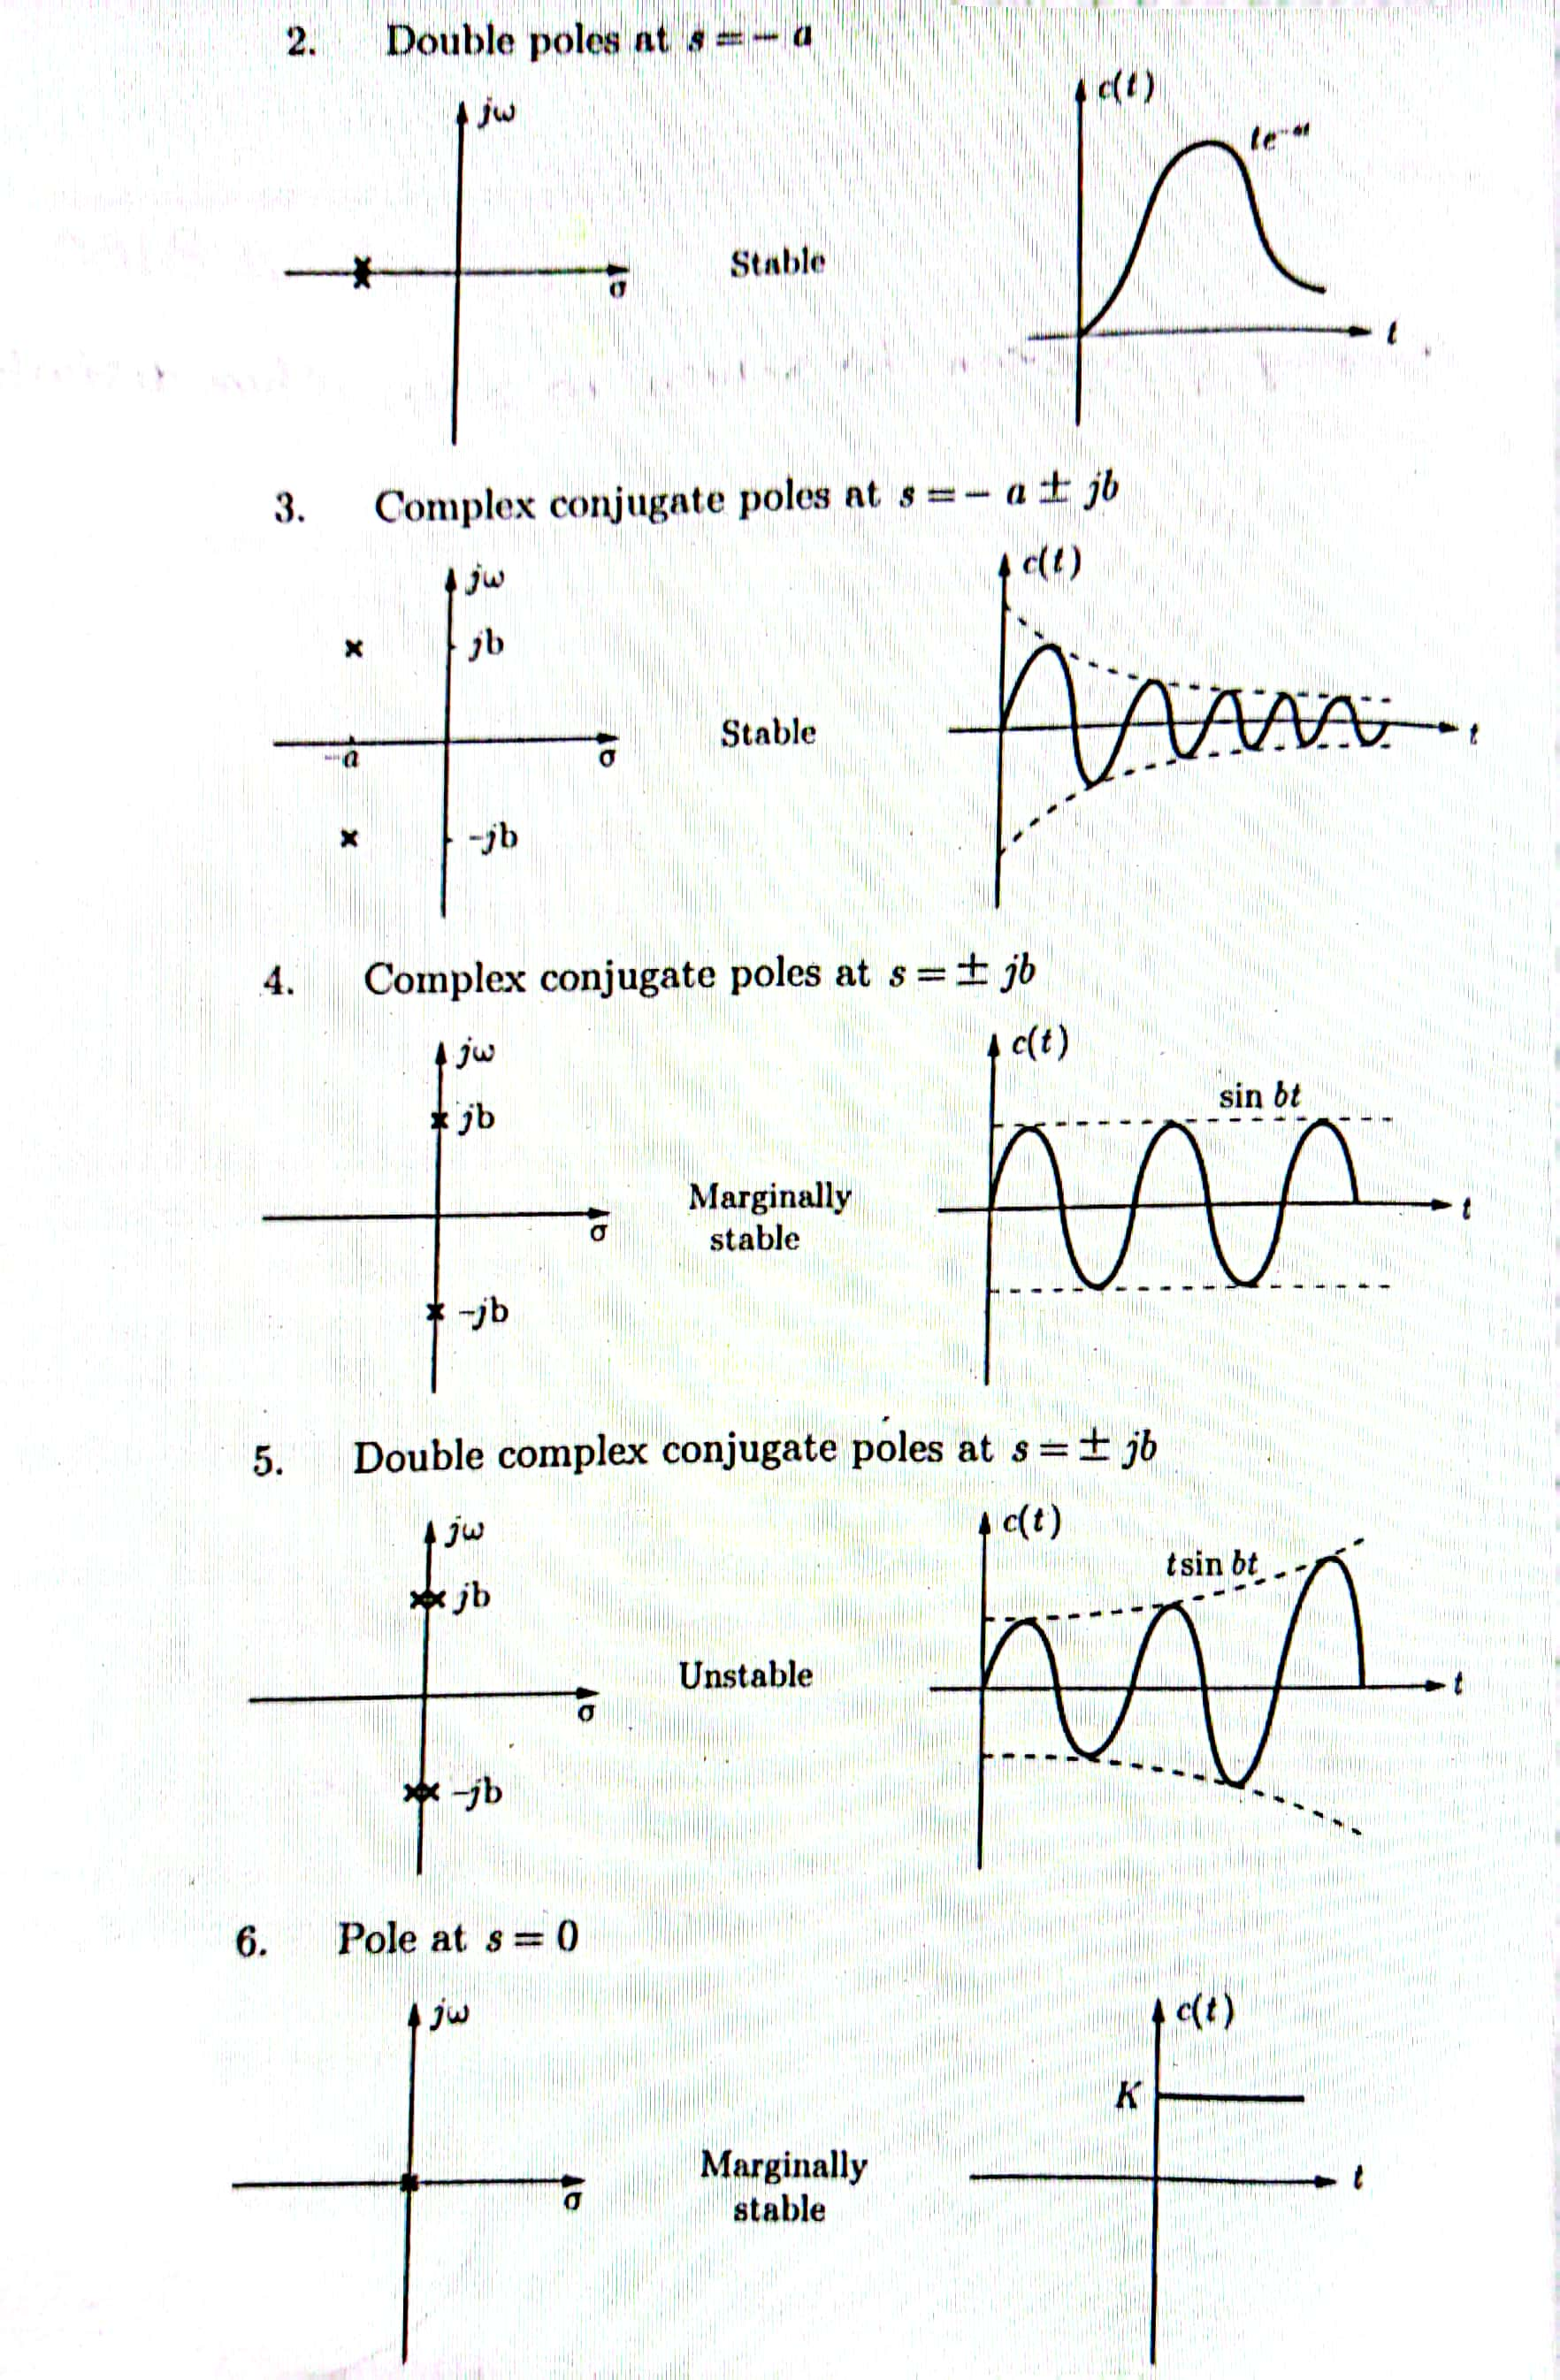
\includegraphics[width=\linewidth]{src/laplace/lpfig1}
\end{figure}
\begin{figure}
	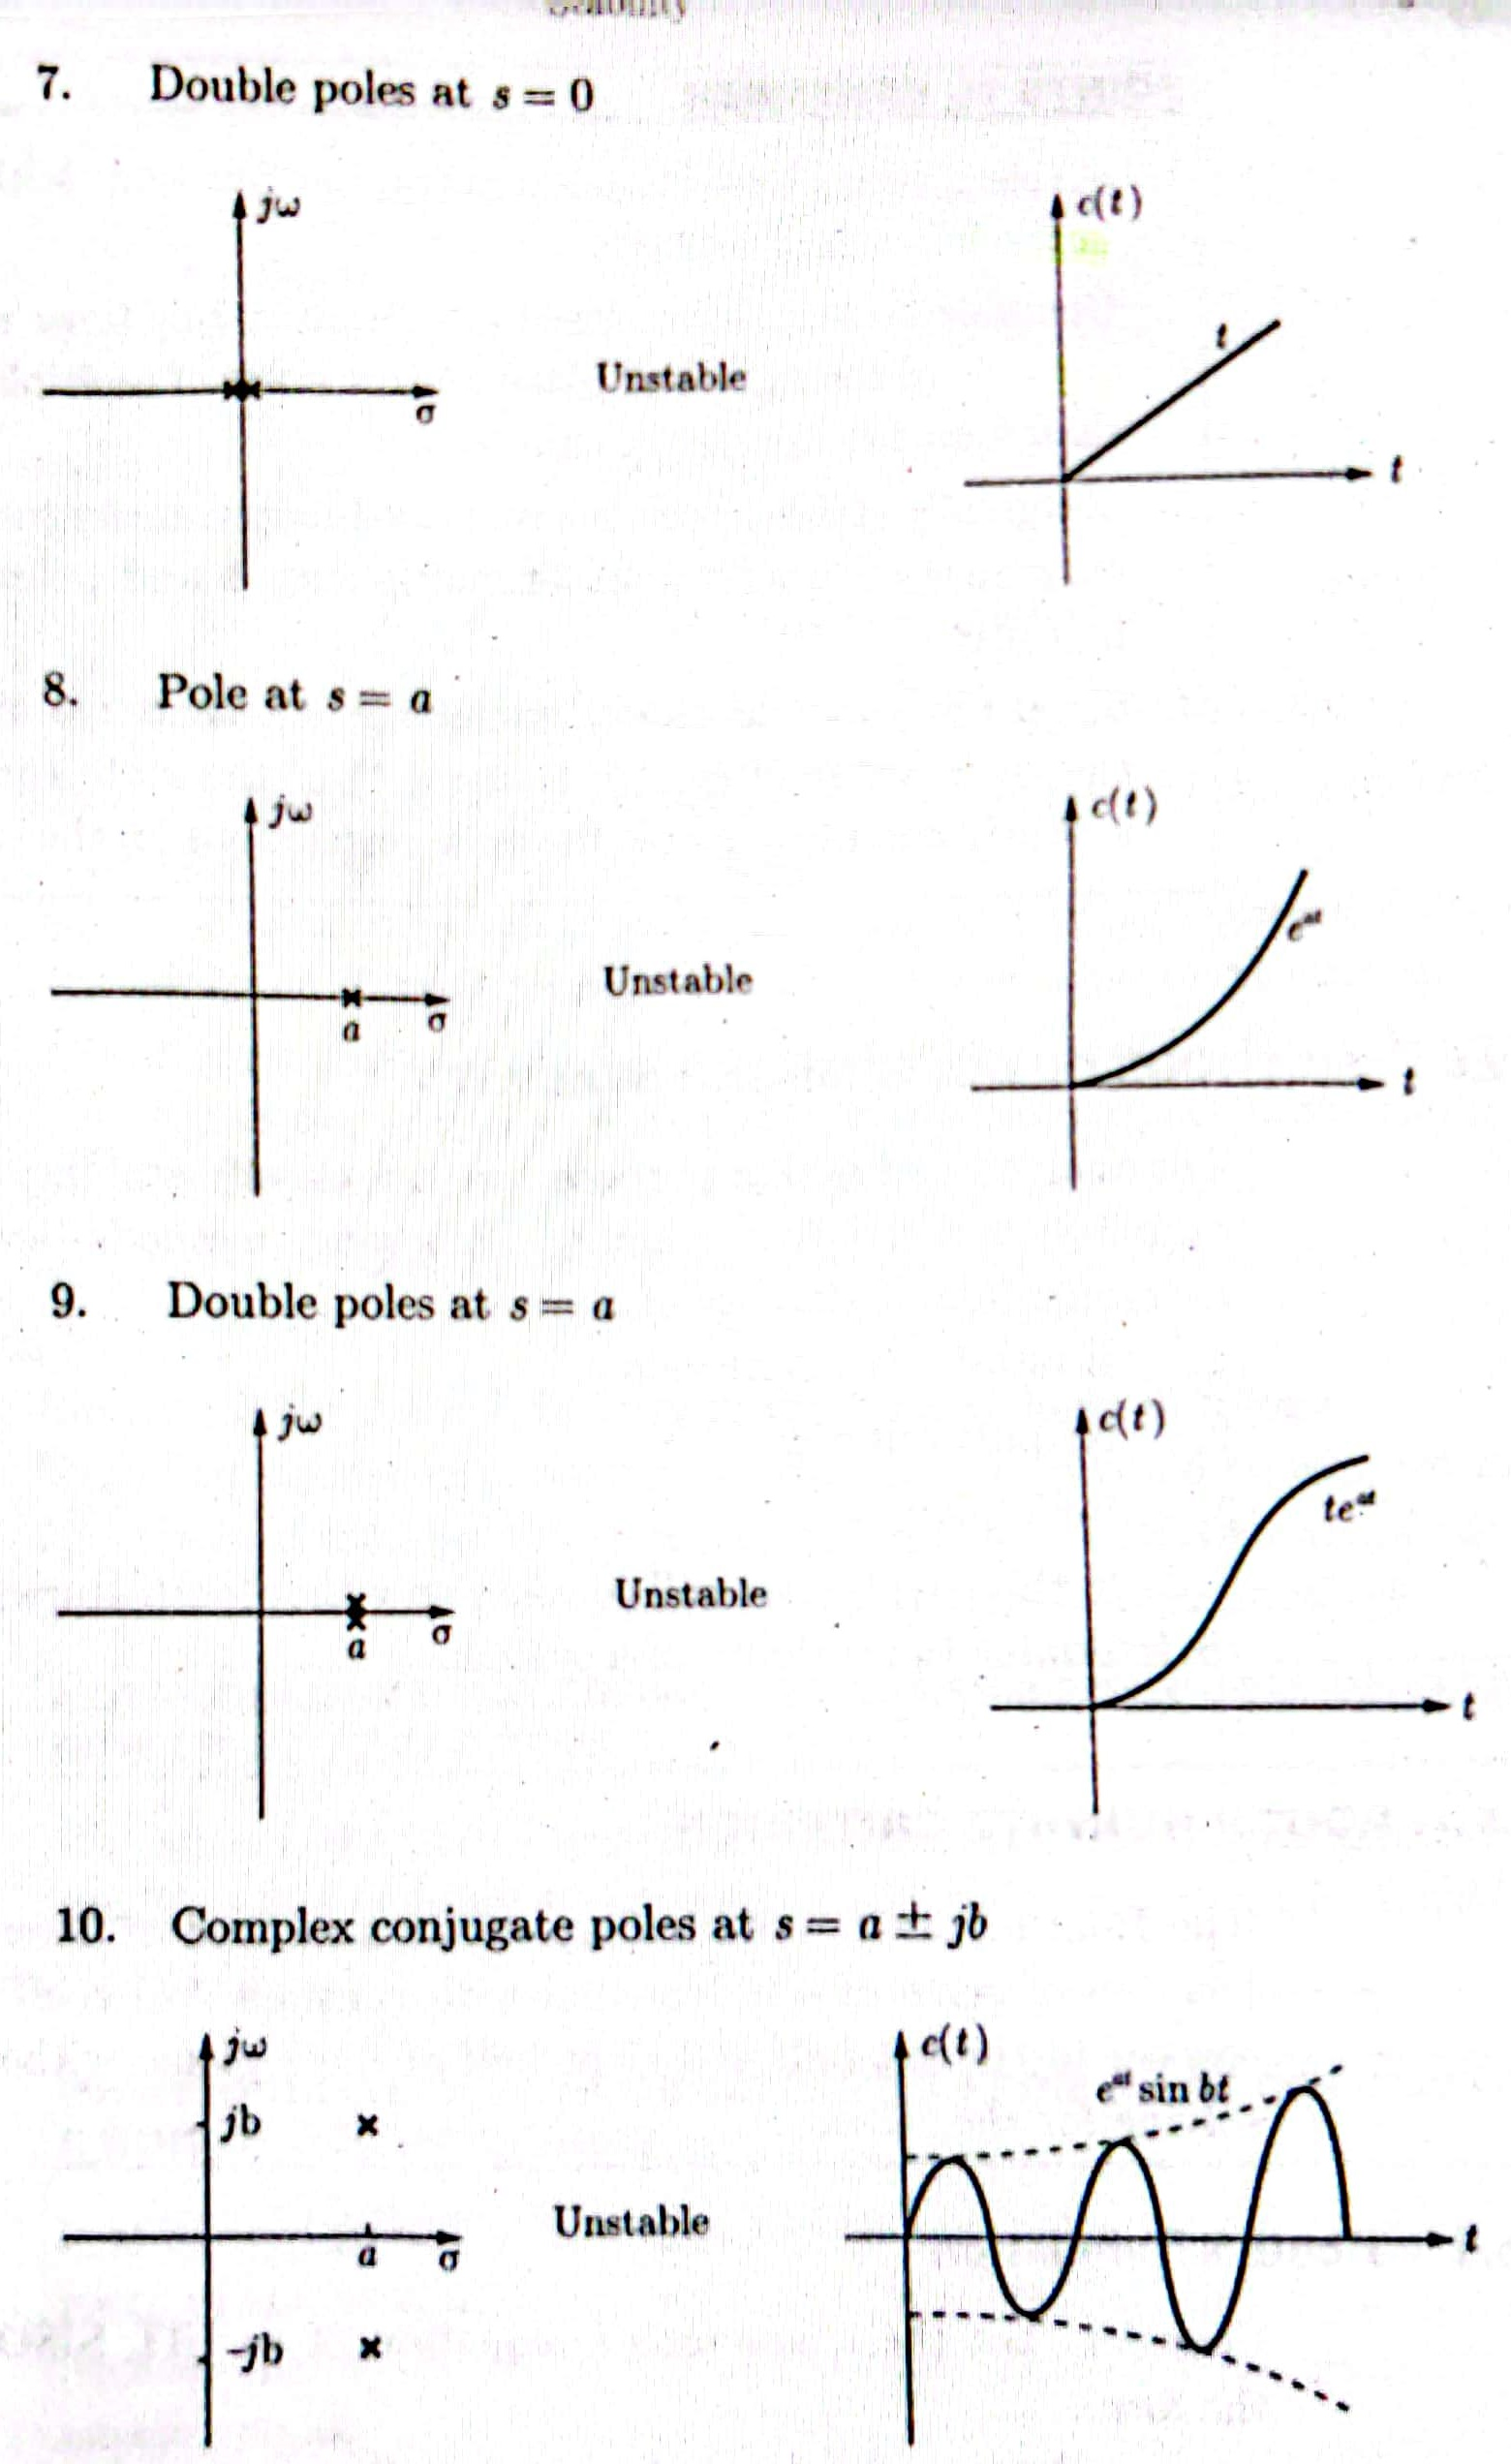
\includegraphics[width=\linewidth]{src/laplace/lpfig2}
\end{figure}

	\chapter{State Space Representation}
Linear State Space Form
\[
\dot{x} = A(t)x+Bu(t)
\]
Non-Linear State Space Form
\[
\dot{x} = f(t,x,u)
\]

\section{Forming State Space}
\begin{tcolorbox}[title=Process]
	\begin{itemize}
		\item Step 1 : Obtain Equation of Motion.
		\item Step 2 : Choose State Variables [ex: position, velocity ...].
		\item Step 3 : Take Derivative of State Vector.
		\item Step 4 : Write in State-Space form
		\item Step 5 : Write Output Equation.
	\end{itemize}
\end{tcolorbox}


\paragraph{Example 1} Obtain S.S from system below
\begin{itemize}
	\item Step 1 : Obtain Equation of Motion.
\end{itemize}
\[
\ddot{y} + 4 \dot{y} + 3 y = 3 u
\]
\begin{itemize}
	\item Step 2 : Choose State Variables. We would like to know \(y\) and \(\dot{y}\). Thus, Let Choose:
\end{itemize}
\[
\begin{split}
	X_1 &= y \\
	X_2 &= \dot{y}
\end{split}
\]
\begin{itemize}
	\item Step 3 : Take Derivative of State Vector.
\end{itemize}
\[
\begin{split}
	X_1 &= y => \dot{X}_1 = \dot{y}\\
	X_2 &= \dot{y} => \dot{X}_2 = \ddot{y} = 3u - 4 \dot{y} - 3 y
\end{split}
\]
\[
\begin{bmatrix}
	\dot{X}_1 \\
	\dot{X}_2 
\end{bmatrix} =
\begin{bmatrix}
	\dot{y}              \\
	3u - 4 \dot{y} - 3 y 
\end{bmatrix}
\]
\begin{itemize}
	\item Step 4 : Write in State-Space form.
\end{itemize}
\[
\dot{X} = 
\begin{bmatrix}
	\dot{X}_1 \\
	\dot{X}_2 
\end{bmatrix} =
\begin{bmatrix}
	0  &   & 1  \\
	-3 &   & -4 
\end{bmatrix}
\begin{bmatrix}
	X_1 \\
	X_2 
\end{bmatrix} +
\begin{bmatrix}
	0 \\
	3 
\end{bmatrix} u
\]
\begin{itemize}
	\item Step 5 : Write Output Equation. We choose \(y=y_{one}\) because we only interest in displacement only \(X_1\), if we are interested in velocity \(X_2\) as well we choose \(y=y_{two}\).
\end{itemize}
\[
y_{one} =
\begin{bmatrix}
	1 &   & 0 
\end{bmatrix}
\begin{bmatrix}
	X_1 \\
	X_2 
\end{bmatrix} \text{or  }
y_{two} = 
\begin{bmatrix}
	1 &   & 0 \\
	0 &   & 1 
\end{bmatrix}
\begin{bmatrix}
	X_1 \\
	X_2 
\end{bmatrix}
\]



\paragraph{Example 2} Obtain S.S from system of mass, spring, damper

\begin{figure}[h]
	\centering
	%\def\svgscale{1}
	\includesvg{src/statespace/statespace_fig1}
\end{figure}

\begin{itemize}
	\item Step 1 : Obtain Equation of Motion. From the 2nd law of Newton:
\end{itemize}
\[
\sum \vec{F} = m\vec{a}
\]
\[
\begin{split}
	F - ky - c \dot{y} &= m \ddot{y} \\
	m \ddot{y} + c \dot{y} + ky &= F \\
	\ddot{y} + \frac{c}{m} \dot{y} + \frac{k}{m} y &= \frac{F}{m}
\end{split}
\]
\begin{itemize}
	\item Step 2 : Choose State Variables. We would like to know \(y\) and \(\dot{y}\). Thus, Let Choose:
\end{itemize}
\[
\begin{split}
	X_1 &= y \\
	X_2 &= \dot{y}
\end{split}
\]
\begin{itemize}
	\item Step 3 : Take Derivative of State Vector.
\end{itemize}
\[
\begin{split}
	X_1 &= y => \dot{X}_1 = \dot{y}\\
	X_2 &= \dot{y} => \dot{X}_2 = \ddot{y} = \frac{F}{m} - \frac{c}{m} \dot{y} - \frac{k}{m} y
\end{split}
\]
\[
\begin{bmatrix}
	\dot{X}_1 \\
	\dot{X}_2 
\end{bmatrix} =
\begin{bmatrix}
	\dot{y}                                           \\
	\frac{F}{m} - \frac{c}{m} \dot{y} - \frac{k}{m} y 
\end{bmatrix}
\]
\begin{itemize}
	\item Step 4 : Write in State-Space form.
\end{itemize}
\[
\dot{X} = 
\begin{bmatrix}
	\dot{X}_1 \\
	\dot{X}_2 
\end{bmatrix} =
\begin{bmatrix}
	0            &   & 1            \\
	\frac{-k}{m} &   & \frac{-c}{m} 
\end{bmatrix}
\begin{bmatrix}
	X_1 \\
	X_2 
\end{bmatrix} +
\begin{bmatrix}
	0           \\
	\frac{1}{m} 
\end{bmatrix} F
\]
\begin{itemize}
	\item Step 5 : Write Output Equation.
\end{itemize}
\[
y =
\begin{bmatrix}
	1 &   & 0 
\end{bmatrix}
\begin{bmatrix}
	X_1 \\
	X_2 
\end{bmatrix}
\]


\paragraph{Example 3} Obtain S.S from system of mass, spring with 2 vertical mass

\begin{figure}[h]
	\centering
	%\def\svgscale{1}
	\includesvg{src/statespace/statespace_fig2}
\end{figure}


\begin{itemize}
	\item Step 1 : Obtain Equation of Motion. From the 2nd law of Newton:
\end{itemize}
\[
\sum \vec{F} = m\vec{a}
\]
\[
\begin{split}
	\text{Mass 1: } -k_1y_1 + k_2y_1 + u_1 + k_2y_2 = m_1\ddot{y}_1 \\
	\text{Mass 2: } -k_3y_2 - k_2y_2 + u_2 + k_2y_1 = m_2\ddot{y}_2
\end{split}
\]
\begin{itemize}
	\item Step 2 : Choose State Variables. We would like to know \(y\) and \(\dot{y}\). Thus, Let Choose:
\end{itemize}
\[
\begin{split}
	X_1 &= y_1 \\
	X_2 &= \dot{y}_1 \\
	X_3 &= y_2 \\
	X_4 &= \dot{y}_2
\end{split}
\]
\begin{itemize}
	\item Step 3 : Take Derivative of State Vector.
\end{itemize}
\[
\begin{split}
	X_1 &= y_1 => \dot{X}_1 = \dot{y}_1 \\
	X_2 &= \dot{y}_1 => \dot{X}_2 = \ddot{y}_1 = -\frac{k_1}{m_1}y_1 + \frac{k_2}{m_1}y_1 + \frac{1}{m_1}u_1 + \frac{k_2}{m_1}y_2 = \frac{k_2 - k_1}{m_1}y_1 + \frac{1}{m_1}u_1 + \frac{k_2}{m_1}y_2 \\
	X_3 &= y_2 => \dot{X}_3 = \dot{y}_2 \\ 
	X_4 &= \dot{y}_2 => \dot{X}_4 = \ddot{y}_2 = -\frac{k_3}{m_2}y_2 - \frac{k_2}{m_2}y_2 + \frac{1}{m_2}u_2 + \frac{k_2}{m_2}y_1 = \frac{-k_3 - k_2}{m_2}y_2 + \frac{1}{m_2}u_2 + \frac{k_2}{m_2}y_1
\end{split}
\]
\[
\begin{bmatrix}
	\dot{X}_1 \\
	\dot{X}_2 \\
	\dot{X}_3 \\
	\dot{X}_4 
\end{bmatrix} =
\begin{bmatrix}
	\dot{y}_1                                                         \\
	\frac{k_2 - k_1}{m_1}y_1 + \frac{1}{m_1}u_1 + \frac{k_2}{m_1}y_2  \\
	\dot{y}_2                                                         \\
	\frac{-k_3 - k_2}{m_2}y_2 + \frac{1}{m_2}u_2 + \frac{k_2}{m_2}y_1 
\end{bmatrix}
\]
\begin{itemize}
	\item Step 4 : Write in State-Space form.
\end{itemize}
\[
\dot{X} = 
\begin{bmatrix}
	\dot{X}_1 \\
	\dot{X}_2 \\
	\dot{X}_3 \\
	\dot{X}_4 
\end{bmatrix} =
\begin{bmatrix}
	0                     &   & 1 &   & 0                      &   & 0 \\
	\frac{k_2 - k_1}{m_1} &   & 0 &   & \frac{k_2}{m_1}        &   & 0 \\
	0                     &   & 0 &   & 0                      &   & 1 \\
	\frac{k_2}{m_2}       &   & 0 &   & \frac{-k_3 - k_2}{m_2} &   & 0 \\
\end{bmatrix}
\begin{bmatrix}
	X_1 \\
	X_2 \\
	X_3 \\
	X_4 
\end{bmatrix} +
\begin{bmatrix}
	0             &   & 0             \\
	\frac{1}{m_1} &   & 0             \\
	0             &   & 0             \\
	0             &   & \frac{1}{m_2} 
\end{bmatrix}
\begin{bmatrix}
	u_1 \\
	u_2 
\end{bmatrix}
\]
\begin{itemize}
	\item Step 5 : Write Output Equation.
\end{itemize}
\[
y =
\begin{bmatrix}
	1 &   & 0 &   & 0 &   & 0 \\ 
	0 &   & 0 &   & 1 &   & 0 \\ 
\end{bmatrix}
\begin{bmatrix}
	X_1 \\
	X_2 \\
	X_3 \\
	X_4 
\end{bmatrix}
\]

\paragraph{Example 4} Solve system of single mass and spring and force using Matlab. 
\begin{lstlisting}[language=MATLAB,title=MATLAB Numerical Method using ode45(Runge Kutta)]
	[t,x] = ode45(@f,tspan,x_0)
	t = time
	x = state vector
	ode45 = solver
	f = function
	tspan = t_0 -> t_f
	x_0 = initial condition
	
	
	Example:
	
	tspan = [0,10];
	x_0 = [0,0];
	
	function dx = model(t,x)
	% dx = Ax+Bu
	k = 0.01;m=1;u=2;
	A = [0 1;-k/m 0];
	B = [0;1/m];
	dx = A*x + B*u;
	
	[t,x] = ode45(@model,tspan,x_0);
	plot(t,x(:;1))
	hold on
	plot(t,x(:;2))
	legend('displacement','velocity')
\end{lstlisting}

\paragraph{Example 5} Obtain S.S from system of mass, spring, damper with 2 horizontal mass

\begin{figure}[h]
	\centering
	%\def\svgscale{1}
	\includesvg{src/statespace/statespace_fig2}
\end{figure}

Equation of Motion
\[
\sum \vec{F} = m\vec{a}
\]
\[
\begin{split}
	\text{Mass 1: }& m_1\ddot{p}(t) + b_1\dot{p}(t) + k_1p(t) = u(t) +k_1q(t)+b_1\dot{q}(t) \\
	\text{Mass 2: }& m_2\ddot{q}(t) + (k_1+k_2)q(t) + (b_1+b_2)\dot{q}(t) = k_1p(t)+b_1\dot{p}(t) \\
	&\ddot{p}(t)= \frac{1}{m_1}u(t) +\frac{k_1}{m_1}q(t)+\frac{b_1}{m_1}\dot{q}(t) - \frac{b_1}{m_1}\dot{p}(t) - \frac{k_1}{m_1}p(t)\\
	&\ddot{q}(t)= \frac{k_1}{m_2}p(t)+\frac{b_1}{m_2}\dot{p}(t) - \frac{(k_1+k_2)}{m_2}q(t) - \frac{(b_1+b_2)}{m_2}\dot{q}(t)
\end{split}
\]
Let:
\[
x = 
\begin{bmatrix}
	x_1 \\
	x_2 \\
	x_3 \\
	x_4 
\end{bmatrix}
= 
\begin{bmatrix}
	p       \\
	q       \\
	\dot{p} \\
	\dot{q} 
\end{bmatrix}
=>
\dot{x} = 
\begin{bmatrix}
	\dot{x}_1 \\
	\dot{x}_2 \\
	\dot{x}_3 \\
	\dot{x}_4 
\end{bmatrix}
= 
\begin{bmatrix}
	\dot{p}  \\
	\dot{q}  \\
	\ddot{p} \\
	\ddot{q} 
\end{bmatrix}
\]
Thus, we get state space form:
\[
\dot{x} = 
\begin{bmatrix}
	\dot{x}_1 \\
	\dot{x}_2 \\
	\dot{x}_3 \\
	\dot{x}_4 
\end{bmatrix} =
\begin{bmatrix}
	0                 &   & 0                       &   & 1                 &   & 0                       \\
	0                 &   & 0                       &   & 0                 &   & 1                       \\
	- \frac{k_1}{m_1} &   & \frac{k_1}{m_1}         &   & - \frac{b_1}{m_1} &   & \frac{b_1}{m_1}         \\
	\frac{k_1}{m_2}   &   & - \frac{(k_1+k_2)}{m_2} &   & \frac{b_1}{m_2}   &   & - \frac{(b_1+b_2)}{m_2} 
\end{bmatrix}
\begin{bmatrix}
	x_1 \\
	x_2 \\
	x_3 \\
	x_4 
\end{bmatrix} +
\begin{bmatrix}
	0             \\
	0             \\
	\frac{1}{m_1} \\
	0             
\end{bmatrix} u(t)
\]

\[
y =
\begin{bmatrix}
	1 &   & 0 &   & 0 &   & 0 
\end{bmatrix}
\begin{bmatrix}
	x_1 \\
	x_2 \\
	x_3 \\
	x_4 
\end{bmatrix}
\]




\section{State Space of Scalar Differential Equation System}

\subsection{Case 1}
Consider equation below:
\[
y^{(n)} + a_1y^{(n-1)} + ... + a_{n-1}y' + a_n y = u  \leftarrow \text{Input has not derivative}
\]
Let:
\[
x = 
\begin{bmatrix}
	x_1     \\
	x_2     \\
	\vdots  \\
	x_{n-1} \\
	x_n     
\end{bmatrix}
=
\begin{bmatrix}
	y       \\
	y'      \\
	\vdots  \\
	y^{n-1} \\
	y^n     
\end{bmatrix}
\]
Thus
\[
\dot{x} = 
\begin{bmatrix}
	\dot{x}_1     \\
	\dot{x}_2     \\
	\vdots        \\
	\dot{x}_{n-1} \\
	\dot{x}_n     
\end{bmatrix}
=
\begin{bmatrix}
	y'                                \\
	y''                               \\
	\vdots                            \\
	y^n                               \\
	-a_0x_1 - a_1x_2 ... - a_nx_n + u 
\end{bmatrix}
=
\begin{bmatrix}
	\dot{x}_2                         \\
	\dot{x}_3                         \\
	\vdots                            \\
	\dot{x}_n                         \\
	-a_0x_1 - a_1x_2 ... - a_nx_n + u 
\end{bmatrix}
\]
Arrange into SS form:
\[
\dot{x} = 
\begin{bmatrix}
	0      &   & 1        &   & 0        &   & ... &   & 0      \\
	0      &   & 0        &   & 1        &   & ... &   & 0      \\
	\vdots &   & \vdots   &   & \vdots   &   & ... &   & \vdots \\
	-a_n   &   & -a_{n-1} &   & -a_{n-2} &   & ... &   & -a_1   
\end{bmatrix}
\begin{bmatrix}
	x_1    \\
	x_2    \\
	\vdots \\
	x_n    
\end{bmatrix} +
\begin{bmatrix}
	0      \\
	0      \\
	\vdots \\
	1      
\end{bmatrix} u
\]
\[
y =
\begin{bmatrix}
	1 &   & 0 &   & ... &   & 0 
\end{bmatrix}
\begin{bmatrix}
	x_1    \\
	x_2    \\
	\vdots \\
	x_n    
\end{bmatrix}
\]
We have a corresponding Transfer Function is 
\[\frac{Y(s)}{U(s)} = \frac{1}{s^n+a_1s^{n-1}+...+a_{n-1}s+a_n}\]

\subsection{Case 2}
Consider equation below:
\[
y^{(n)} + a_1y^{(n-1)} + ... + a_{n-1}y' + a_n y = \beta_0u^n + \beta_1u^{n-1}+ ... +\beta_nu  \leftarrow \text{Input has derivative}
\]
Let:
\[
\begin{split}
	x_1 &= y - \beta_0 u \\
	x_2 &= y' - \beta_0 u' - \beta_1 u = x'_1-\beta_1u \\
	\vdots \\
	x_n &= y^{n-1} - \beta_0 u^{n-1} - ... - \beta_{n-1} u = x'_{n-1}-\beta_{n-1}u
\end{split}
\]
Where \(\beta_0 , \beta_1 , ... , \beta_{n-1}\) are determined from:
\[
\begin{split}
	\beta_0 &= b_0 \\
	\beta_1 &= b_1 - a_1\beta_0 \\
	\beta_2 &= b_2 - a_1\beta_1 - a_2\beta_0 \\
	\vdots
\end{split}
\]
Arrange into SS form:
\[
\dot{x} = 
\begin{bmatrix}
	0      &   & 1        &   & 0        &   & ... &   & 0      \\
	0      &   & 0        &   & 1        &   & ... &   & 0      \\
	\vdots &   & \vdots   &   & \vdots   &   & ... &   & \vdots \\
	-a_n   &   & -a_{n-1} &   & -a_{n-2} &   & ... &   & -a_1   
\end{bmatrix}
\begin{bmatrix}
	x_1    \\
	x_2    \\
	\vdots \\
	x_n    
\end{bmatrix} +
\begin{bmatrix}
	\beta_1 \\
	\beta_2 \\
	\vdots  \\
	\beta_n 
\end{bmatrix} u
\]
\[
y =
\begin{bmatrix}
	1 &   & 0 &   & ... &   & 0 
\end{bmatrix}
\begin{bmatrix}
	x_1    \\
	x_2    \\
	\vdots \\
	x_n    
\end{bmatrix} + \beta_0 u
\]
We have a corresponding Transfer Function is 
\[\frac{Y(s)}{U(s)} = \frac{b_0 s^n + b_1s^{n-1} + ... + b_{n-1}s+ b_n}{s^n+a_1s^{n-1}+...+a_{n-1}s+a_n}\]


\section{Transfer Function to State Space}
\paragraph{Example}
\[\frac{Y(s)}{U(s)} = \frac{100}{s^4 + 20s^3 + 10s^2 + 7s + 100}\]
\[(s^4 + 20s^3 + 10s^2 + 7s + 100)Y(s) = 100 U(s)\]
Taking Inverse Laplace Transform
\[y^{(4)} + 20y^{(3)} + 10 y'' + 7y' + 100y = 100 u\]
Let:
\[
\begin{split}
	x_1 &= y   => \dot{x}_1 = y' = x_2\\
	x_2 &= y'  => \dot{x}_2 = y'' = x_3\\
	x_3 &= y'' => \dot{x}_3 = y^{(3)} = x_4\\
	x_3 &= y'''=> \dot{x}_4 = y^{(4)} = 100u - 20y^{(3)} - 10 y'' - 7y' - 100y
\end{split}
\]
State Space form:
\[
\dot{x} = 
\begin{bmatrix}
	0    &   & 1  &   & 0   &   & 0   \\
	0    &   & 0  &   & 1   &   & 0   \\
	0    &   & 0  &   & 0   &   & 1   \\
	-100 &   & -7 &   & -10 &   & -20 
\end{bmatrix}
\begin{bmatrix}
	x_1 \\
	x_2 \\
	x_3 \\
	x_4 
\end{bmatrix} + 
\begin{bmatrix}
	0   \\
	0   \\
	0   \\
	100 
\end{bmatrix} u
\]
\[
y =
\begin{bmatrix}
	1 &   & 0 &   & 0 &   & 0 
\end{bmatrix}
\begin{bmatrix}
	x_1 \\
	x_2 \\
	x_3 \\
	x_4 
\end{bmatrix}
\]


\section{State Space to Transfer Function}
We have a Transfer Function:
\[
\frac{Y(s)}{U(s)} = G(s)
\]
with state space in form of:
\[
\begin{split}
	\dot{x} &= Ax + Bu \\
	y &= Cx + Du
\end{split}
\]
Let have a Laplace transform of SS:
\[
\begin{split}
	sX(s)-x(0) &= AX(s) + BU(s) \\
	Y(s) &= CX(s) + DU(s)
\end{split}
\]
Assuming \(x(0) = 0 IC\), we get:
\[
\begin{split}
	sX(s) - AX(s) &= BU(s) \\
	(sI - A)X(s) &= BU(s) \\
	(sI - A)^{-1}(sI - A)X(s) &= (sI - A)^{-1}BU(s) \\
	X(s) &= (sI - A)^{-1}BU(s)
\end{split}
\]
Substitute into \(Y(s)\)
\[
\begin{split}
	Y(s) &= C[(sI - A)^{-1}BU(s)] + DU(s) \\
	Y(s) &= C(sI - A)^{-1}BU(s) + DU(s) \\
	Y(s) &= [C(sI - A)^{-1}B + D]U(s)
\end{split}
\]
Thus the Transfer function can be found by:
\[
G(s) = C(sI - A)^{-1}B + D
\]


\paragraph{Example}
\[
\dot{x} = 
\begin{bmatrix}
	0  &   & 1   &   & 0  \\
	0  &   & 0   &   & 1  \\
	-5 &   & -25 &   & -5 
\end{bmatrix}
\begin{bmatrix}
	x_1 \\
	x_2 \\
	x_3 
\end{bmatrix} + 
\begin{bmatrix}
	0    \\
	25   \\
	-120 
\end{bmatrix} u
\]
\[
y =
\begin{bmatrix}
	1 &   & 0 &   & 0 
\end{bmatrix}
\begin{bmatrix}
	x_1 \\
	x_2 \\
	x_3 
\end{bmatrix}
\]

\[
G(s) = 
\begin{bmatrix}
	1 &   & 0 &   & 0 
\end{bmatrix}
[
\begin{bmatrix}
	s &   & 0 &   & 0 \\
	0 &   & s &   & 0 \\
	0 &   & 0 &   & s 
\end{bmatrix}
-
\begin{bmatrix}
	0  &   & 1   &   & 0  \\
	0  &   & 0   &   & 1  \\
	-5 &   & -25 &   & -5 
\end{bmatrix}]^{-1}
\begin{bmatrix}
	0    \\
	25   \\
	-120 
\end{bmatrix} + 0
\]

\[
G(s) = 
\begin{bmatrix}
	1 &   & 0 &   & 0 
\end{bmatrix}
\begin{bmatrix}
	s  &   & 1   &   & 0   \\
	0  &   & s   &   & 1   \\
	-5 &   & -25 &   & s+5 
\end{bmatrix}^{-1}
\begin{bmatrix}
	0    \\
	25   \\
	-120 
\end{bmatrix}
\]

\[
G(s) = 
\begin{bmatrix}
	1 &   & 0 &   & 0 
\end{bmatrix}
\begin{bmatrix}
	\frac{(s^2+5s+25)}{(s^3+5s^2+25s-5)} &   & \frac{(-s-5)}{(s^3+5s^2+25s-5)}   &   & \frac{1}{(s^3+5s^2+25s-5)}   \\
	\frac{-5}{(s^3+5s^2+25s-5)}          &   & \frac{(s^2+5s)}{(s^3+5s^2+25s-5)} &   & \frac{-s}{(s^3+5s^2+25s-5)}  \\
	\frac{5s}{(s^3+5s^2+25s-5)}          &   & \frac{(25s-5)}{(s^3+5s^2+25s-5)}  &   & \frac{s^2}{(s^3+5s^2+25s-5)} 
\end{bmatrix}
\begin{bmatrix}
	0    \\
	25   \\
	-120 
\end{bmatrix}
\]

\[
G(s) = 
\begin{bmatrix}
	1 &   & 0 &   & 0 
\end{bmatrix}
\begin{bmatrix}
	\frac{(-25s-245)}{(s^3+5s^2+25s-5)}         \\
	\frac{(25s^2+245s)}{(s^3+5s^2+25s-5)}       \\
	\frac{(-120s^2+625s-125)}{(s^3+5s^2+25s-5)} 
\end{bmatrix}
\]

\[
G(s) = \frac{(-25s-245)}{(s^3+5s^2+25s-5)}
\]


Thus
\[
G(s) = \frac{25s + 245}{s^3 + 5s^2 + 25s + 5}
\]
	\chapter{Linear Approximation with Taylor Series}
What is a Linear System ?
Linear System is a system that comply to 2 rules.
\begin{itemize}
	\item Superposition (Addition).
	\item Homogeneous (Multiplication). 
\end{itemize}

\section{Superposition}


Given that we have a function \(y = f(x)\).
\begin{itemize}
	\item If we have a value \(x_1\) substitute to the function we get \(y_1\) : \(y_1 = f(x_1)\)
	\item If we have a value \(x_2\) substitute to the function we get \(y_1\) : \(y_2 = f(x_2)\).
	\item If we have a value \(x_1 + x_2\) substitute to the function we should get \(y_1+y_2\) : \(y_1+y_2 = f(x_1+x_2)\)
\end{itemize}

\section{Homogeneous}

Given that we have a function \(y = f(x)\).
\begin{itemize}
	\item If we have a value \(\alpha x_1\) substitute to the function we get \(y_1\) : \(y_1 = f(\alpha x_1)\)
	\item If we have a value \(x_1\) substitute to the function then multiply by \(\alpha\) we should get \(y_1 = \alpha f(x_1)\)
\end{itemize}

\paragraph{Example} Find out if the function is linear : \(y = x\)
\paragraph{Superposition test} \(y_1 = x_1, y_2 = x_2\)
Add both result together \(y_1 + y_2 = x_1 + x_2\) \\
Substitute \(x_1 + x_2\) to the function we get \(y_1+y_2\). Thus, \(y_1+y_2=y_{12}\). TEST PASS.

\paragraph{Homogeneous test} Substitute \(\alpha x\) we get \(y = \alpha x\).
Substitute \(x\) and multiply by \(\alpha\) we get \(y = \alpha x\). Thus, \(\alpha x=\alpha x\). TEST PASS. Both test is passed and thus the system is linear.


\paragraph{Example} Find out if the function is linear : \(y = x^2\)
\paragraph{Superposition test}\(y_1 = x_1^2, y_2 = x_2^2\). Add both result together \(y_1 + y_2 = x_1^2 + x_2^2\). Substitute \(x_1 + x_2\) to the function we get \((x_1+x_2)^2\). Thus, \(y_1+y_2!=y_{12}\). TEST FAIL. The test is failed and thus the system is nonlinear.

\section{Linearization Process}
One of the Linearization method is by using Tyler Expansion Series within an operational range for stability.
\[
y \approx y(x_0) + \left[\frac{dy}{dx}|_{x_0}\frac{(x-x_0)}{1!}\right] + \left[\frac{d^2y}{dx^2}|_{x_0}\frac{(x-x_0)^2}{2!}\right] + ... [Higher Order Term]
\]
Let take a look at the plot:

\begin{figure}[h]
\centering
%		\def\svgscale{1}
\includesvg{src/tyler/tyler}
\caption{Mass spring system}
\label{fig:Plot}
\end{figure}

\(y=L(x)\) is the linear approximation of \(y=f(x)\) and \(a = x_0\) is an equilibrium point. We can see that we want to pick an operational range where the function is stable because the \(y=L(x)\) is close to \(y=f(x)\). As we move a way from the operational range, the approximation is starting to diverge from the real solution.


\paragraph{Example} Linearize : \(y = x^2\).
We have:
\[
y \approx y(x_0) + \left[\frac{dy}{dx}|_{x_0}\frac{(x-x_0)}{1!}\right] + \left[\frac{d^2y}{dx^2}|_{x_0}\frac{(x-x_0)^2}{2!}\right] + ... [Higher Order Term]
\]
Only consider the first order term and eliminate HOT because in HOT the variable \(x\) is subject to power number that will make it nonlinear. We get:
\[
y \approx y(x_0) + \left[\frac{dy}{dx}|_{x_0}\frac{(x-x_0)}{1!}\right]
\]
We get:
\[
\frac{dy}{dx}|_{x_0} = \frac{d(x^2)}{dx}|_{x_0} = 2x|_{x_0} = 2x_0
\]
We get:
\[
\begin{split}
	y &\approx y(x_0) + \left[2x_0\frac{(x-x_0)}{1!}\right]\\
	y &\approx y(x_0) + \left[2x_0(x-x_0)\right]
\end{split}
\]
\[
\boxed{y \approx y(x_0) + 2x_0x-2x_0^2}
\]
Let pick an equilibrium point \(x_0=2\)
\[
\begin{split}
	y &= 2^2 + 2\times2x-2\times2^2 \\
	y &= 4+4x-8 \\
	y &= 4x-4
\end{split}
\]
Now that we have a original function \(y=x^2\) and approximation function at \(x_0 = 2\) \(y=4x-4\). Let compare:
\[
\begin{split}
	x &= 2 \\
	=>y_{ori} &= 2^2 = 4 \\
	=>y_{lin} &= 4\times2 - 4 = 4
\end{split}
\]
Both are equal to each other at equilibrium point.
\[
\begin{split}
	x &= 3 \\
	=>y_{ori} &= 3^2 = 9 \\
	=>y_{lin} &= 4\times3 - 4 = 8
\end{split}
\]
A way from the equilibrium point, it starts to diverge.
	
	\chapter{DC Motor}
DC motor is a mechatronic product that consist of two parts: the mechanical part and the electrical part. A typical dc motor used by a robot is constructed by: a dc motor, a wheel encoder (for measuring rotation pulse of motor ), and a gear box (for reducing the speed of motor).


\begin{figure}[ht]
	\centering
	%\def\svgscale{1}
	\includesvg{src/dcmotor/dcmotor_fig1}
	\caption{Typical DC Motor}
	\label{fig:dcmotor}
\end{figure}

\section{Modelling}

\begin{figure}[ht]
	\centering
	%\def\svgscale{1}
	\includesvg{src/dcmotor/dcmotor_fig2}
	\caption{dc motor model}
	\label{fig:dc motor model}
\end{figure}

\subsection{Electrical Part}
\begin{equation}
	v_b(t) = K_b \dot{\theta}(t) = K_b \omega(t)
	\label{dcmotoreq1}
\end{equation}
Where:
\begin{itemize}
	\item {\makebox[1cm]{\(v_b(t)\)\hfill} is voltage at terminal conductor of motor }
	\item {\makebox[1cm]{\(K_b\)\hfill} is back emf constant}
	\item {\makebox[1cm]{\(\dot{\theta} = \omega\)\hfill} is angular velocity of motor}
\end{itemize}

\begin{equation}
	T_a = K_t i_a(t)
	\label{dcmotoreq2}
\end{equation}
Where:
\begin{itemize}
	\item {\makebox[1cm]{\(T_a\)\hfill} is rotor torque }
	\item {\makebox[1cm]{\(K_t\)\hfill} is motor torque}
	\item {\makebox[1cm]{\(i_a\)\hfill} is the current draw by motor}
\end{itemize}
\hfill\\
By applying Kirchoff Voltage Law to the circuit loop in \autoref{fig:dc motor model}
\begin{itemize}
	\item {\makebox[3.5cm]{\(v_a(t)\)\hfill} is input voltage from power source}
	\item {\makebox[3.5cm]{\(v_{resistance} = R_a i_a(t)\)\hfill} is voltage across resistance}
	\item {\makebox[3.5cm]{\(v_{inductor} = L_a \frac{di_a(t)}{dt}\)\hfill} is voltage across inductor}
\end{itemize}

\[v_a(t) - v_b(t) - R_a i_a(t) - L_a \frac{di_a(t)}{dt} = 0\]

\begin{equation}
	\Rightarrow v_a(t) = v_b(t) + R_a i_a(t) + L_a \frac{di_a(t)}{dt}
	\label{dcmotoreq3}
\end{equation}
Substitute \autoref{dcmotoreq1} into \autoref{dcmotoreq3}, we get:

\begin{equation}
	v_a(t) = K_b \omega(t) + R_a i_a(t) + L_a \frac{di_a(t)}{dt}
	\label{dcmotoreq4}
\end{equation}
In practical dc motor the \(L_a\) is very small (\(L_a \approx 0\)) and neglectable.

\[v_a(t) = K_b \omega(t) + R_a i_a(t)\]

\begin{equation}
	\Rightarrow \boxed{i_a(t) = \frac{v_a(t) - K_b \omega(t)}{R_a}}
	\label{dcmotoreq5}
\end{equation}

\subsection{Mechanical Part}

\begin{equation}
	T_a = T_f + J \dot{\omega}(t)
	\label{dcmotoreq6}
\end{equation}
Where:
\begin{itemize}
	\item {\makebox[1cm]{\(T_f\)\hfill} is torque of coulomb friction and viscous friction }
	\item {\makebox[1cm]{\(J\)\hfill} is moment of inertia}
\end{itemize}
We know that:
\begin{equation}
	T_f = T_c sign[\omega(t)]+D\omega(t)
	\label{dcmotoreq7}
\end{equation}
Where:
\begin{itemize}
	\item {\makebox[1cm]{\(T_c\)\hfill} is coulomb friction torque}
	\item {\makebox[1cm]{\(D\)\hfill} is coefficient viscous friction}
\end{itemize}
Substitute \autoref{dcmotoreq7} to \autoref{dcmotoreq6}, we get:
\[T_a = T_c sign[\omega(t)]+D\omega(t) + J \dot{\omega}(t)\]

\subsection{Approximation of coulomb friction to zero \(T_c \approx 0\)}
\begin{equation}
	T_a = D\omega(t) + J \dot{\omega}(t)
	\label{dcmotoreq8}
\end{equation}
From \autoref{dcmotoreq2}: \(T_a = K_t i_a(t)\) substitute to \autoref{dcmotoreq8}:
\[K_t i_a(t) = D\omega(t) + J \dot{\omega}(t)\]
\begin{equation}
	\Rightarrow \boxed{i_a(t) = \frac{D\omega(t) + J \dot{\omega}(t)}{K_t}}
	\label{dcmotoreq9}
\end{equation}

\subsection{Keep coulomb friction \(T_c\)}
\begin{equation}
	\Rightarrow \boxed{i_a(t) = \frac{T_c sign[\omega(t)] + D\omega(t) + J \dot{\omega}(t)}{K_t}}
	\label{dcmotoreq10}
\end{equation}

\subsection{Electrical and Mechanical combine}
\subsection{Approximation of coulomb friction to zero \(T_c \approx 0\)}

From \autoref{dcmotoreq5} and \autoref{dcmotoreq9}: Put it side by side:

\[i_a(t) = i_a(t)\]
\[\frac{v_a(t) - K_b \omega(t)}{R_a} = \frac{D\omega(t) + J \dot{\omega}(t)}{K_t}\]
Get \(\dot{\omega}(t)\):

\[\dot{\omega}(t) = \frac{\frac{(v_a(t) - K_b \omega(t))K_t}{R_a} - D\omega(t)}{J}\]
\[\dot{\omega}(t) = \frac{(v_a(t) - K_b \omega(t))K_t}{R_a J} - \frac{D\omega(t)}{J}\]
\[\dot{\omega}(t) = \frac{v_a(t) K_t - K_b K_t\omega(t)}{R_a J} - \frac{D\omega(t)}{J}\]
Separate \(\omega(t)\) and \(v_a(t)\):

\begin{tcolorbox}[title=Lumped Parameters without Friction]
	\begin{equation}
		\dot{\omega}(t) = - (\frac{K_b K_t + D R_a}{R_a J})\omega(t) + \frac{K_t}{R_a J}v_a(t)
		\label{dcmotoreq11}
	\end{equation}
	Let:
	\begin{itemize}
		\item {\makebox[4cm]{\(a = (\frac{K_b K_t + D R_a}{R_a J}) \omega(t)\)\hfill} \([1/s]\) }
		\item {\makebox[4cm]{\(b = \frac{K_t}{R_a J}\)\hfill} \([rad/s^2/V]\) }
	\end{itemize}
	We get lumped Parameter in a simplified form as:
	\begin{equation}
		\Rightarrow \dot{\omega}(t) = - a\omega(t) + bv_a(t)
		\label{dcmotoreq12}
	\end{equation}
\end{tcolorbox}



\subsection{Keep coulomb friction \(T_c\)}
\begin{tcolorbox}[title=Lumped Parameters with Friction]
	\begin{equation}
		\dot{\omega}(t) = - (\frac{K_b K_t + D R_a}{R_a J})\omega(t) + \frac{K_t}{R_a J}v_a(t) - \frac{T_c}{J}sign(\omega(t))
		\label{dcmotoreq13}
	\end{equation}
	Let:
	\begin{itemize}
		\item {\makebox[4cm]{\(a = (\frac{K_b K_t + D R_a}{R_a J})\)\hfill} \([1/s]\) }
		\item {\makebox[4cm]{\(b = \frac{K_t}{R_a J}\)\hfill} \([rad/s^2/V]\) }
		\item {\makebox[4cm]{\(c = \frac{T_c}{J}\)\hfill} \([.]\) }
	\end{itemize}
	We get lumped Parameter in a simplified form as:
	\begin{equation}
		\Rightarrow \dot{\omega}(t) = - a\omega(t) + bv_a(t) - csign(\omega(t))
		\label{dcmotoreq14}
	\end{equation}
\end{tcolorbox}


\section{Simulation}

In general, the equation \(\dot{\omega}(t) = - a\omega(t) + bv_a(t) - csign(\omega(t)\) is used to represent all the dc motor in the market. By modifying the parameters \(a, b, c\) will result in different dc motor.
From equation \(\dot{\omega}(t) = - a\omega(t) + bv_a(t) - csign(\omega(t))\)
\begin{itemize}
	\item {\makebox[1cm]{\(\dot{\omega}(t)\)\hfill} is the angular acceleration of dc motor and is the output of the system}
	\item {\makebox[1cm]{\(\omega(t)\) \hfill} is the angular velocity of dc motor and is the output of the system}
	\item {\makebox[1cm]{\(v_a(t)\)\hfill} is the input voltage to dc motor and is the input of the system}
\end{itemize}

\begin{figure}[ht]
	\centering
	%def\svgscale{1}
	\includesvg{src/dcmotor/dcmotor_fig3}
	\caption{Simulation Flow}
	\label{fig:Simulation Flow}
\end{figure}


\section{DC Motor 2nd Order Model ($ L_a $ is not Neglected)}
\subsection{No Friction}
From \autoref{dcmotoreq4} and \autoref{dcmotoreq9}, we have:
\[\begin{split}
	v_a(t) &= K_b \omega(t) + R_a i_a(t) + L_a \frac{di_a(t)}{dt} \\
	i_a(t) &= \frac{D\omega(t) + J \dot{\omega}(t)}{K_t}
\end{split}\]
\[\begin{split}
	\frac{di_a(t)}{d(t)} &= \frac{d}{dt}\left(\frac{D\omega(t) + J \dot{\omega}(t)}{K_t}\right) \\
	&= \frac{1}{K_t}\frac{d}{dt}(D\omega(t) + J \dot{\omega}(t))\\
	&= \frac{1}{K_t} \frac{d}{dt}(D\omega(t)) + \frac{d}{dt}(J \dot{\omega}(t)) \\
	&= \frac{1}{K_t} (D\dot{\omega}(t) + J \ddot{\omega}(t))
\end{split}\]
We get:
\begin{equation}
	v_a(t) = K_b \omega(t) + R_a \frac{D\omega(t) + J \dot{\omega}(t)}{K_t} + L_a\frac{1}{K_t} (D\dot{\omega}(t) + J \ddot{\omega}(t))
	\label{dcmotoreq15}
\end{equation}
\[\begin{split}
	K_tv_a(t) &= K_tK_b \omega(t) + R_a (D\omega(t) + J \dot{\omega}(t)) + L_a (D\dot{\omega}(t) + J \ddot{\omega}(t)) \\
	K_tv_a(t) &= K_tK_b \omega(t) + R_a D\omega(t) + R_a J \dot{\omega}(t) + L_a D\dot{\omega}(t) + L_aJ \ddot{\omega}(t) \\
	K_tv_a(t) &= (K_tK_b + R_a D) \omega(t) + (R_a J + L_a D) \dot{\omega}(t) + L_aJ \ddot{\omega}(t) \\
	L_aJ \ddot{\omega}(t) &= -(K_tK_b + R_a D) \omega(t) - (R_a J + L_a D) \dot{\omega}(t) + K_tv_a(t) \\
\end{split}\]
\begin{tcolorbox}[title=Lumped Parameters without Friction 2nd Order]
	\[\ddot{\omega}(t) = - \frac{R_a J + L_a D}{L_aJ} \dot{\omega}(t) -\frac{K_tK_b + R_a D}{L_aJ} \omega(t)  + \frac{K_t}{L_aJ}v_a(t)\]
	Let:
	\[
	a = \frac{R_a J + L_a D}{L_aJ} , b = \frac{K_tK_b + R_a D}{L_aJ} , c = \frac{K_t}{L_aJ}
	\]
	We get lumped Parameter in a simplified form as:
	\begin{equation}
		\Rightarrow \ddot{\omega}(t) = - a\dot{\omega}(t) - b\omega(t) + cv_a(t)
		\label{dcmotoreq16}
	\end{equation}
\end{tcolorbox}


\subsection{With Friction}
From \autoref{dcmotoreq4} and \autoref{dcmotoreq10}, we have:
\[\begin{split}
	v_a(t) &= K_b \omega(t) + R_a i_a(t) + L_a \frac{di_a(t)}{dt} \\
	i_a(t) &= \frac{T_c sign[\omega(t)] +D\omega(t) + J \dot{\omega}(t)}{K_t}
\end{split}\]
\[\begin{split}
	\frac{di_a(t)}{d(t)} &= \frac{d}{dt}\left(\frac{T_c sign[\omega(t)] +D\omega(t) + J \dot{\omega}(t)}{K_t}\right) \\
	&= \frac{1}{K_t} (D\dot{\omega}(t) + J \ddot{\omega}(t)) \leftarrow \text{derivative of sign function is 0}
\end{split}\]
We get:
\begin{equation}
	v_a(t) = K_b \omega(t) + R_a \frac{T_c sign[\omega(t)] + D\omega(t) + J \dot{\omega}(t)}{K_t} + L_a\frac{1}{K_t} (D\dot{\omega}(t) + J \ddot{\omega}(t))
	\label{dcmotoreq17}
\end{equation}
\[
K_tv_a(t) = K_tK_b \omega(t) + R_aT_c sign[\omega(t)] + R_aD\omega(t) + R_aJ \dot{\omega}(t)) + L_a D\dot{\omega}(t) + L_a J \ddot{\omega}(t)
\]

\begin{tcolorbox}[title=Lumped Parameters with Friction 2nd Order]
	\[
	\ddot{\omega}(t) = - \frac{R_a J + L_a D}{L_aJ} \dot{\omega}(t) -\frac{K_tK_b + R_a D}{L_aJ} \omega(t)  + \frac{K_t}{L_aJ}v_a(t) - \frac{R_aT_c}{L_aJ} sign[\omega(t)]
	\]
	Let:
	\[
	a = \frac{R_a J + L_a D}{L_aJ}, b = \frac{K_tK_b + R_a D}{L_aJ}, c = \frac{K_t}{L_aJ}, d = \frac{R_aT_c}{L_aJ}
	\]
	We get lumped Parameter in a simplified form as:
	\begin{equation}
		\Rightarrow \ddot{\omega}(t) = - a\dot{\omega}(t) - b\omega(t) + cv_a(t) - dsign(\omega(t))
		\label{dcmotoreq18}
	\end{equation}
\end{tcolorbox}

	\chapter{DC Motor Lamped Parameters Identification}
DC Motor is widely used in many applications such as robot, industrial application -etc. It has been produced in great number, some is at high standard with larger documentation and specification while some are inexpensive with little to none of documentation. To be able to use the dc motor efficiently, we must know it mathematical model. In this lesson, we use a variant of a famous algorithm known as Extended Kalman Filter (EKF) and Unscented Kalman Filter (UKF) to estimate the dc motor model.\par

\section{DC Motor Stochastic State Space Model}
	From Lecture 1 : DC Motor, We have a mathematical model to represent the motor:\\
	Model with neglect the coulomb friction:
	\[\boxed{\dot{\omega}(t) = - a\omega(t) + bv_a(t)}\]
	Model with the coulomb friction:
	\[\boxed{\dot{\omega}(t) = - a\omega(t) + bv_a(t) - csign(\omega(t))}\]

\subsection{Model with neglect the coulomb friction}
	From the model:
	\begin{equation}
		\dot{\omega}(t) = - a \omega(t) + b v_a(t)
		\label{dcmotorideq1}
	\end{equation}
	In control system, we have a state space model for a nonlinear model:
	\[\dot{x}(t) = f(t,x(t),u(t)) + v_{noise}(t)\]
	\[y(t) = h(t,x(t),u(t)) + \omega_{noise}(t)\]
	Where:
	\begin{itemize}
		\item {\makebox[1cm]{\(\dot{x}(t)\)\hfill} is rate of change of state }
		\item {\makebox[1cm]{\(x(t)\)\hfill} is the current state}
		\item {\makebox[1cm]{\(u(t)\)\hfill} is the input to the system}
		\item {\makebox[1cm]{\(y(t)\)\hfill} is the measurement model}
		\item {\makebox[1.5cm]{\(v_{noise}(t)\)\hfill} is random process noise}
		\item {\makebox[1.5cm]{\(\omega_{noise}(t)\)\hfill} is random measurement noise}
	\end{itemize}
	From \autoref{dcmotorideq1}, Let:
	\begin{equation}
		\begin{split}
			x_1 = \omega\\
			x_2 = a\\
			x_3 = b
		\end{split}
		\label{dcmotorideq2}
	\end{equation}
	We get:
	\begin{equation}
		\begin{split}
			\dot{x_1} = \dot{\omega} = - a \omega(t) + b v_a(t) &= -x_2 x_1 + x_3 v_a(t)\\
			\dot{x_2} &= 0 \\
			\dot{x_3} &= 0
		\end{split}
		\label{dcmotorideq3}
	\end{equation}
	
	\begin{tcolorbox}[title=In continuous nonlinear stochastic system matrix form]
		\begin{equation}
			\begin{split}
					\dot{x}(t) =
					\begin{bmatrix}
						\dot{x_1} \\
						\dot{x_2} \\
						\dot{x_3} 
					\end{bmatrix}(t) &=
					\begin{bmatrix}
						-x_2 x_1 + x_3 v_a(t) \\
						0                     \\
						0                     
					\end{bmatrix} +\sqrt{Q_c}v_{noise}(t)\\
					y(t) &= 
					\begin{bmatrix}
						1 & 0 & 0 
					\end{bmatrix}
					\begin{bmatrix}
						x_1 \\
						x_2 \\
						x_3 
					\end{bmatrix}(t)+\sqrt{R}\omega_{noise}(t)
			\end{split}
			\label{dcmotorideq4}
		\end{equation}
	\end{tcolorbox}
	
	
	Discretize the continuous model from \autoref{dcmotorideq4}:
	\begin{equation}
		\begin{split}
			\dot{x}(t) &=
			\begin{bmatrix}
				-x_2 x_1 + x_3 v_a(t) \\
				0                     \\
				0                     
			\end{bmatrix} +\sqrt{Q_c}v_{noise}(t)\\
			y(t) &= 
			\begin{bmatrix}
				1 & 0 & 0 
			\end{bmatrix}
			\begin{bmatrix}
				x_1 \\
				x_2 \\
				x_3 
			\end{bmatrix}(t)+\sqrt{R}\omega_{noise}(t)
		\end{split}
		\label{dcmotorideq5}
	\end{equation}
	\begin{equation}
		\begin{split}
			\frac{x_{k+1} - x_k}{T_s} &=
			\begin{bmatrix}
				-x_2 x_1 + x_3 v_a(t) \\
				0                     \\
				0                     
			\end{bmatrix} +\sqrt{Q_c}v_{noise}(t)\\
			y_k &= 
			\begin{bmatrix}
				1 & 0 & 0 
			\end{bmatrix}
			\begin{bmatrix}
				x_1 \\
				x_2 \\
				x_3 
			\end{bmatrix}_k+\sqrt{R}\omega_{noise}(t)
		\end{split}
		\label{dcmotorideq6}
	\end{equation}

	\begin{tcolorbox}[title=Discretized nonlinear stochastic system in matrix form]
		\begin{equation}
			\begin{split}
					x_{k+1} &= x_k + T_s
					\begin{bmatrix}
						-x_2 x_1 + x_3 v_{a,k} \\
						0                      \\
						0                      
					\end{bmatrix} +\sqrt{T_s Q_d}v_{noise,k}\\
					y_k &= 
					\begin{bmatrix}
						1 & 0 & 0 
					\end{bmatrix}
					\begin{bmatrix}
						x_1 \\
						x_2 \\
						x_3 
					\end{bmatrix}_k+\sqrt{R}\omega_{noise,k}
			\end{split}
			\label{dcmotorideq7}
		\end{equation}
	\end{tcolorbox}
	

\subsection{Model the coulomb friction}
	From the model:
	\begin{equation}
		\dot{\omega}(t) = - a \omega(t) + b v_a(t) - csign(\omega(t))
		\label{dcmotorideq8}
	\end{equation}
	From \autoref{dcmotorideq8}, Let:
	\begin{equation}
		\begin{split}
			x_1 = \omega\\
			x_2 = a\\
			x_3 = b\\
			x_4 = c
		\end{split}
		\label{dcmotorideq9}
	\end{equation}
	We get:
	\begin{equation}
		\begin{split}
			\dot{x_1} = \dot{\omega} = - a \omega(t) + b v_a(t) &= -x_2 x_1 + x_3 v_a(t) - x_4sign(x_1)  \\
			\dot{x_2} &= 0 \\
			\dot{x_3} &= 0 \\
			\dot{x_4} &= 0
		\end{split}
		\label{dcmotorideq10}
	\end{equation}

	
	\begin{tcolorbox}[title=In continuous nonlinear stochastic system matrix form]
		\begin{equation}
			\begin{split}
					\dot{x}(t) =
					\begin{bmatrix}
						\dot{x_1} \\
						\dot{x_2} \\
						\dot{x_3} \\
						\dot{x_4} 
					\end{bmatrix}(t) &=
					\begin{bmatrix}
						-x_2 x_1 + x_3 v_a(t) - x_4sign(x_1) \\
						0                                    \\
						0                                    \\
						0                                    
					\end{bmatrix} +\sqrt{Q_c}v_{noise}(t)\\
					y(t) &= 
					\begin{bmatrix}
						1 & 0 & 0 & 0 
					\end{bmatrix}
					\begin{bmatrix}
						x_1 \\
						x_2 \\
						x_3 \\
						x_4 
					\end{bmatrix}(t)+\sqrt{R}\omega_{noise}(t)
			\end{split}
			\label{dcmotorideq11}
		\end{equation}
	\end{tcolorbox}
	
	
	\begin{tcolorbox}[title=Discretized nonlinear stochastic system in matrix form]
		\begin{equation}
			\begin{split}
					x_{k+1} &= x_k + T_s
					\begin{bmatrix}
						-x_2 x_1 + x_3 v_{a,k} - x_4sign(x_1) \\
						0                                     \\
						0                                     \\
						0                                     
					\end{bmatrix} +\sqrt{T_s Q_d}v_{noise,k}\\
					y_k &= 
					\begin{bmatrix}
						1 & 0 & 0 & 0 
					\end{bmatrix}
					\begin{bmatrix}
						x_1 \\
						x_2 \\
						x_3 \\
						x_4 
					\end{bmatrix}_k+\sqrt{R}\omega_{noise,k}
			\end{split}
			\label{dcmotorideq12}
		\end{equation}
	\end{tcolorbox}
	

	\section{Identification using Extended Kalman Filter (EKF)}
	
	\begin{tcolorbox}[title=DC Motor Parameters Identification with EKF]
		\paragraph{Initialize} Select any
		\begin{itemize}
			\item {\makebox[1cm]{\(\hat{x}_{0|0}\)\hfill} initial state estimate}
			\item {\makebox[1cm]{\(P_{0|0}\)\hfill} positive definite error covariance matrix}
		\end{itemize}
		\paragraph{Time Update}
		\begin{equation}
			\begin{split}
				\hat{x}_{k+1|k} &= f_d(\hat{x}_{k|k},u_k)\\
				P_{k+1|k} &= A_kP_{k|k}A^T_k+Q
			\end{split}
			\label{dcmotorideq13}
		\end{equation}
		\paragraph{Measurement Update}
		\begin{equation}
			\begin{split}
				\hat{y}_{k+1|k} &= h_d(\hat{x}_{k+1|k},u_{k+1})\\
				P_{xz,k+1|k}    &= P_{k+1|k}C^T_{k+1}\\
				P_{zz,k+1|k}    &= C_{k+1}P_{k+1|k}C^T_{k+1}+R\\
				\hat{x}_{k+1|k+1} &= \hat{x}_{k+1|k} + P_{xz,k+1|k}P^{-1}_{zz,k+1|k}(y_{k+1}-\hat{y}_{k+1|k})\\
				P_{k+1|k+1}     &= P_{k+1|k} - P_{xz,k+1|k}P^{-1}_{zz,k|k+1}P^T_{xz,k+1|k} 
			\end{split}
			\label{dcmotorideq14}
		\end{equation}
	\end{tcolorbox}
	
	
	\subsection{Model with neglect the coulomb friction}
	From \autoref{dcmotorideq7}, We have:
	\[\begin{split}
		x_{k+1} &= x_k + T_s
		\begin{bmatrix}
			-x_2 x_1 + x_3 v_{a,k} \\
			0                      \\
			0                      
		\end{bmatrix} +\sqrt{T_s Q_d}v_{noise,k}\\
		y_k &= 
		\begin{bmatrix}
			1 & 0 & 0 
		\end{bmatrix}
		\begin{bmatrix}
			x_1 \\
			x_2 \\
			x_3 
		\end{bmatrix}_k+\sqrt{R}\omega_{noise,k}
	\end{split}\]


	\begin{center}
		\textbf{Applying Extended Kalman Filter}
	\end{center}
	\paragraph{Initialize} state and positive definite error covariance matrix
	\[\begin{split}
		\hat{x}_{0|0} &= \begin{bmatrix}
			2 \\
			13 \\
			25
		\end{bmatrix} \text{ or some number randomly}\\
		P_{0|0} &= 2*eye(3) = 
		\begin{bmatrix}
			2 & 0 & 0 \\
			0 & 2 & 0 \\
			0 & 0 & 2 
		\end{bmatrix} \text{ or some number randomly}
	\end{split}\]
	
	\paragraph{Time Update}
	\begin{itemize}
		\item {\makebox[2cm]{\(T_s = 0.01\)\hfill} sampling time (s) , up to user}
		\item \(Q = 0.00001
		\begin{bmatrix}
			10 & 0  & 0  \\
			0  & 25 & 0  \\
			0  & 0  & 25 
		\end{bmatrix} 
		= 0.00001 \times diag([10\quad 25\quad 25])\) \\process covariance matrix, smaller is truth in process model (use for tuning)
		\item \(R = 0.02
		\begin{bmatrix}
			1 & 0 & 0 \\
			0 & 1 & 0 \\
			0 & 0 & 1 
		\end{bmatrix} 
		= 0.02 \times diag([1\quad 1\quad 1])\) \\measurement covariance matrix, smaller is truth in measurement (use for tuning)
	\end{itemize}

	\paragraph{Compute} \[\hat{x}_{k+1|k} = \hat{x}_k + T_s
	\begin{bmatrix}
		-x_2 x_1 + x_3 v_{a,k} \\
		0                      \\
		0                      
	\end{bmatrix} + \boxed{\sqrt{T_s Q_d}v_{noise,k}}\]
	$\sqrt{T_s Q_d}v_{noise,k}$ put this bunch if we use in simulation to simulate noise to a true system, don't put if taking real value from system because the system has noise already.
	
	\paragraph{Compute}
	\[P_{k+1|k} = A_kP_{k|k}A^T_k+Q\]
	where:
	\[A_k =
	\begin{bmatrix}
		-x_2 & -x_1 & v_a \\
		0    & 0    & 0   \\
		0    & 0    & 0   
	\end{bmatrix}\]
	is the jacobian matrix calculated by derivative the state model. From \autoref{dcmotorideq4}
	\[J_f(x,y) =\begin{bmatrix}
		\frac{df_1}{dx_1} & \frac{df_1}{dx_2} & \frac{df_1}{dx_3} \\
		\frac{df_2}{dx_1} & \frac{df_2}{dx_2} & \frac{df_2}{dx_3} \\
		\frac{df_3}{dx_1} & \frac{df_3}{dx_2} & \frac{df_3}{dx_3}
	\end{bmatrix} = 
	\begin{bmatrix}
		\frac{-x_2x_1+x_3v_a}{dx_1} & \frac{-x_2x_1+x_3v_a}{dx_2} & \frac{-x_2x_1+x_3v_a}{dx_3} \\
		\frac{0}{dx_1}              & \frac{0}{dx_2}              & \frac{0}{dx_3}              \\
		\frac{0}{dx_1}              & \frac{0}{dx_2}              & \frac{0}{dx_3}              
	\end{bmatrix}
	\]
	
	
	\paragraph{Measurement Update}
	\paragraph{Compute} \(\hat{y}_{k+1|k} = h_d(\hat{x}_{k+1|k},u_{k+1})\) measurement estimation. This equation is the estimation of a measurement would look like. In our case, we measure the $\omega$ directly (\autoref{dcmotorideq4}) and thus we can take:
	\[\hat{y}_{k+1|k} = [1\quad 0\quad 0]\hat{x}_{k+1|k} + D_ku_{a,k}\]
	Where: \(D_k = 0\)
	\paragraph{Compute} \[
	\begin{split}
		P_{xz,k+1|k} &= P_{k+1|k}C^T_{k+1}\\
		P_{zz,k+1|k} &= C_{k+1}P_{k+1|k}C^T_{k+1}+R
	\end{split}\]
	From \autoref{dcmotorideq4}, we have \(C = [1\quad 0\quad 0]\)

	\paragraph{Compute}
	\[\hat{x}_{k+1|k+1} = \hat{x}_{k+1|k} + P_{xz,k+1|k}P^{-1}_{zz,k+1|k}(y_{k+1}-\hat{y}_{k+1|k})\]
	Where $y_{k+1}$ is the measurement from sensor which has noise mixed inside. Get data directly from the sensor.

	\paragraph{Compute}
	\[P_{k+1|k+1} = P_{k+1|k} - P_{xz,k+1|k}P^{-1}_{zz,k|k+1}P^T_{xz,k+1|k}\]
	
	
	
	
	\subsection{Model with coulomb friction}
	From \autoref{dcmotorideq12}, We have:
	\[
	\begin{split}
		x_{k+1} &= x_k + T_s
		\begin{bmatrix}
			-x_2 x_1 + x_3 v_{a,k} - x_4sign(x_1) \\
			0                                     \\
			0                                     \\
			0                                     
		\end{bmatrix} +\sqrt{T_s Q_d}v_{noise,k}\\
		y_k &= 
		\begin{bmatrix}
			1 & 0 & 0 & 0 
		\end{bmatrix}
		\begin{bmatrix}
			x_1 \\
			x_2 \\
			x_3 \\
			x_4 
		\end{bmatrix}_k+\sqrt{R}\omega_{noise,k}
	\end{split}
	\]
	
	\begin{center}
		\textbf{Applying Extended Kalman Filter}
	\end{center}

	\paragraph{Initialize} state and positive definite error covariance matrix
	\[\begin{split}
		\hat{x}_{0|0} &= \begin{bmatrix}
			2 \\
			13 \\
			25 \\
			1
		\end{bmatrix} \text{ or some number randomly}\\
		P_{0|0} &= 2*eye(4) = 
		\begin{bmatrix}
			2 & 0 & 0 & 0 \\
			0 & 2 & 0 & 0 \\
			0 & 0 & 2 & 0 \\
			0 & 0 & 0 & 2 \\
		\end{bmatrix} \text{ or some number randomly}
	\end{split}\]
	
	\paragraph{Time Update}
	\begin{itemize}
		\item {\makebox[2cm]{\(T_s = 0.01\)\hfill} sampling time (s) , up to user}
		\item \(Q = 0.00001
		\begin{bmatrix}
			10 & 0  & 0  & 0 \\
			0  & 25 & 0  & 0 \\
			0  & 0  & 25 & 0 \\
			0  & 0  & 0  & 1 
		\end{bmatrix} 
		= 0.00001 \times diag([10\quad 25\quad 25\quad 1])\) \\process covariance matrix, smaller is truth in process model (use for tuning)
		\item \(R = 0.02
		\begin{bmatrix}
			1 & 0 & 0 & 0 \\
			0 & 1 & 0 & 0 \\
			0 & 0 & 1 & 0 \\
			0 & 0 & 0 & 1 
		\end{bmatrix} 
		= 0.02 \times diag([1\quad 1\quad 1\quad 1])\) \\measurement covariance matrix, smaller is truth in measurement (use for tuning)
	\end{itemize}
	\paragraph{Compute} \[\hat{x}_{k+1|k} = \hat{x}_k + T_s
	\begin{bmatrix}
		-x_2 x_1 + x_3 v_{a,k} - x_4sign(x_1) \\
		0                                     \\
		0                                     \\
		0                                     
	\end{bmatrix} + \boxed{\sqrt{T_s Q_d}v_{noise,k}}\]
	\paragraph{Compute}
	\[P_{k+1|k} = A_kP_{k|k}A^T_k+Q\]
	where:
	\[A_k =
	\begin{bmatrix}
		-x_2 & -x_1 & v_a & -sign(x_1) \\
		0    & 0    & 0   & 0          \\
		0    & 0    & 0   & 0          \\
		0    & 0    & 0   & 0          
	\end{bmatrix}\]
	is the jacobian matrix calculated by derivative the state model from \autoref{dcmotorideq11}.
	\\
	\paragraph{Measurement Update}
	\paragraph{Compute}
	\[\hat{y}_{k+1|k} = [1\quad 0\quad 0\quad 0]\hat{x}_{k+1|k} + D_ku_{a,k}\]
	Where: \(D_k = 0\)
	\paragraph{Compute} \[
	\begin{split}
		P_{xz,k+1|k} &= P_{k+1|k}C^T_{k+1}\\
		P_{zz,k+1|k} &= C_{k+1}P_{k+1|k}C^T_{k+1}+R
	\end{split}\]
	From \autoref{dcmotorideq11}, we have \(C = [1\quad 0\quad 0\quad 0]\)
	
	\paragraph{Compute}
	\[\hat{x}_{k+1|k+1} = \hat{x}_{k+1|k} + P_{xz,k+1|k}P^{-1}_{zz,k+1|k}(y_{k+1}-\hat{y}_{k+1|k})\]
	Where \(y_{k+1}\) is the measurement from sensor which has noise mixed inside. Get data directly from the sensor.

	\paragraph{Compute}
	\[P_{k+1|k+1} = P_{k+1|k} - P_{xz,k+1|k}P^{-1}_{zz,k|k+1}P^T_{xz,k+1|k}\]
	
	
	
	
	
	
	
	
	\begin{lstlisting}[language=MATLAB]
		function x_est = EKF(uk,y_true)
		Ts=0.01;
		persistent x_est_p P Qd_est R_est Qc_est;
		if isempty(x_est_p)
		x_est_p = [2;13;25;1];
		
		P = 2*[1 0 0 0;
		0 1 0 0;
		0 0 1 0;
		0 0 0 1;]                         %2*eye(4);
		
		Qc_est = 1e-5*[10  0   0  0;
		0  25   0  0;
		0   0  25  0;
		0   0   0  1;]               %1e-5*diag([10,25,25,1]);
		
		Qd_est=Qc_est*Ts;
		
		R_est=0.02;
		end
	
		c=[1 0 0 0]; D=0; Ck=c;	Dk=D;
		
		%Comput Kalman Gain and update predicted value
		Wk=P*Ck'/(Ck*P*Ck'+R_est);
		
		y_est=Ck*x_est_p+Dk*uk;
		
		x=x_est_p+Wk.*(y_true-y_est);
		
		%Compute prediction at next time step
		x_est=x+Ts*[-x(2)*x(1)+uk*x(3)-x(4)*sign(x(1));
		0                 ;
		0                 ;
		0                ];
		
		%Update error covariance matrices
		P=P-Wk*Ck*P;
		
		%Define Ak
		Ak=eye(4)+Ts*[-x(2) -x(1) uk -sign(x(1));
		0     0    0      0     ;
		0     0    0      0     ;
		0     0    0      0     ]; % jacobian
		
		P=Ak*P*Ak'+Qd_est;
		
		x_est_p=x_est;
	\end{lstlisting}
	\chapter{DC Motor Control}
In application of DC Motor, we want to be able to control its position and angular velocity.

\section{Velocity Control using PI Control}
In this section we design a controller for dcmotor based on linearized dcmotor model using 2nd Order Differential Equation Design Workflow. From DC motor Model, we have:
\begin{equation}
	\label{dcmotorctrleq1}
	\dot{\omega}(t) = -a\omega(t) + bv_a(t) 	
\end{equation}
We have to design a velocity controller, thus the feedback of the system is angular velocity of the dc motor.\\
We have our PI control:
\begin{equation}
	\label{dcmotorctrleq2}
	v_a(t) = K_p(\omega_d(t) - \omega(t)) + K_i \int_{0}^{t} (\omega_d(t) - \omega(t)) \,dt
\end{equation}
From \autoref{dcmotorctrleq1},we get:
\begin{equation}
	\label{dcmotorctrleq3}
	v_a(t) = \frac{1}{b}\dot{\omega}_d(t) + \frac{a}{b}\omega_d(t)
\end{equation}
From \autoref{dcmotorctrleq2} and \autoref{dcmotorctrleq3}, we have our controller design:
\begin{equation}
	\label{dcmotorctrleq4}
	v_a(t) = \frac{1}{b}\dot{\omega}_d(t) + \frac{a}{b}\omega_d(t) + K_p(\omega_d(t) - \omega(t)) + K_i \int_{0}^{t} (\omega_d(t) - \omega(t)) \,dt
\end{equation}

\begin{figure}[h]
	\centering
	%\def\svgscale{1}
	\includesvg{src/dcmotorctrl/dcmotorctrl_fig1}
	\caption{Velocity Control PI Controller}
	\label{fig:Velocity Control PI Controller}
\end{figure}

Substitute \autoref{dcmotorctrleq4} back to model in \autoref{dcmotorctrleq1}, we get:
\begin{equation}
	\label{dcmotorctrleq5}
	\dot{\omega}(t) = -a\omega(t) + b\left(\frac{1}{b}\dot{\omega}_d(t) + \frac{a}{b}\omega_d(t) + K_p(\omega_d(t) - \omega(t)) + K_i \int_{0}^{t} (\omega_d(t) - \omega(t)) \,dt\right)
\end{equation}
\[
\begin{split}
	0 &= -\dot{\omega}(t) - a\omega(t) + \dot{\omega}_d(t) + a\omega_d(t) + bK_p(\omega_d(t) - \omega(t)) + bK_i \int_{0}^{t} (\omega_d(t) - \omega(t)) \,dt \\
	0 &= (\dot{\omega}_d(t) - \dot{\omega}(t)) + a(\omega_d(t) - \omega(t)) + bK_p(\omega_d(t) - \omega(t)) + bK_i \int_{0}^{t} (\omega_d(t) - \omega(t)) \,dt \\
	0 &= (\dot{\omega}_d(t) - \dot{\omega}(t)) + (a + bK_p)(\omega_d(t) - \omega(t)) + bK_i \int_{0}^{t} (\omega_d(t) - \omega(t)) \,dt \\
	0 &= \dot{e}_{\omega} + (a + bK_p)e_{\omega} + bK_i \int_{0}^{t} e_{\omega}\,dt \\
	0 &= \ddot{e}_{\omega} + (a + bK_p)\dot{e}_{\omega} + bK_ie_{\omega} \leftarrow \text{take derivative to cancel integral.}\\
\end{split}
\]
Thus, we get:
\begin{equation}
	\label{dcmotorctrleq6}
	\ddot{e}_{\omega} + (a + bK_p)\dot{e}_{\omega} + bK_ie_{\omega} = 0
\end{equation}
From 2nd Order differential equation standard form, we have:
\begin{equation}
	\label{dcmotorctrleq7}
	\ddot{X} + 2\zeta\omega_nX+\omega_n^2X = 0
\end{equation}
From \autoref{dcmotorctrleq6} and \autoref{dcmotorctrleq7}, we get:
\[
\begin{split}
	a + bK_p &= 2\zeta\omega_n \\
	bK_i     &= \omega_n^2 \\
	K_p      &= \frac{2\zeta\omega_n - a}{b} \\
	K_i      &= \frac{\omega_n^2}{b}
\end{split}
\]
From equation above, we want \(K_p > 0\). Thus, \(2\zeta\omega_n > a\), then \(\zeta\omega_n > \frac{a}{2}\) to ensure stability.

\begin{tcolorbox}[title=Velocity Control using PI Linear]
	\paragraph{Control input}
	\[v_a(t) = \frac{1}{b}\dot{\omega}_d(t) + \frac{a}{b}\omega_d(t) + K_p(\omega_d(t) - \omega(t)) + K_i \int_{0}^{t} (\omega_d(t) - \omega(t)) \,dt\]
	\paragraph{Control Tuning Constant}
	\[
	\begin{split}
		K_p      &= \frac{2\zeta\omega_n - a}{b} \\
		K_i      &= \frac{\omega_n^2}{b}
	\end{split}
	\]
\end{tcolorbox}

\section{Velocity Control using PID Control}
In this section we design a controller for dcmotor based on linearized dcmotor model using 2nd Order Differential Equation Design Workflow. From DC motor Model, We have our PID control:
\begin{equation}
	\label{dcmotorctrleq8}
	v_a(t) = K_p(\omega_d(t) - \omega(t)) + K_i \int_{0}^{t} (\omega_d(t) - \omega(t)) \,dt + K_d \frac{d}{dt} (\omega_d(t) - \omega(t))
\end{equation}
From \autoref{dcmotorctrleq3} and \autoref{dcmotorctrleq8}, we have our controller design:
\begin{equation}
	\label{dcmotorctrleq9}
	v_a(t) = \frac{1}{b}\dot{\omega}_d(t) + \frac{a}{b}\omega_d(t) + K_p(\omega_d(t) - \omega(t)) + K_i \int_{0}^{t} (\omega_d(t) - \omega(t)) \,dt + K_d \frac{d}{dt} (\omega_d(t) - \omega(t))
\end{equation}
Substitute \autoref{dcmotorctrleq9} back to model in \autoref{dcmotorctrleq1}, we get:
\begin{equation}
	\label{dcmotorctrleq10}
	\dot{\omega} = -a\omega + b\left(\frac{1}{b}\dot{\omega}_d + \frac{a}{b}\omega_d + K_p(\omega_d - \omega) + K_i \int_{0}^{t} (\omega_d - \omega) \,dt + K_d \frac{d}{dt} (\omega_d - \omega) \right)
\end{equation}
\[
\begin{split}
	0 &= -\dot{\omega} -a\omega + b(\frac{1}{b}\dot{\omega}_d + \frac{a}{b}\omega_d + K_p(\omega_d - \omega) + K_i \int_{0}^{t} (\omega_d - \omega) \,dt + K_d \frac{d}{dt} (\omega_d - \omega)) \\
	0 &= -\dot{\omega} -a\omega + \dot{\omega}_d + a\omega_d + bK_p(\omega_d - \omega) + bK_i \int_{0}^{t} (\omega_d - \omega) \,dt + bK_d \frac{d}{dt} (\omega_d - \omega) \\
	0 &= (\dot{\omega}_d -\dot{\omega}) + (a+bK_p)(\omega_d -\omega) + bK_i \int_{0}^{t} (\omega_d - \omega) \,dt + bK_d \frac{d}{dt} (\omega_d - \omega) \\
	0 &= (1+bK_d)(\dot{\omega}_d -\dot{\omega}) + (a+bK_p)(\omega_d -\omega) + bK_i \int_{0}^{t} (\omega_d - \omega) \,dt \\
	0 &= (1+bK_d)\dot{e}_{\omega} + (a+bK_p)e_{\omega} + bK_i \int_{0}^{t} e_{\omega} \,dt \\
	0 &= (1+bK_d)\ddot{e}_{\omega} + (a+bK_p)\dot{e}_{\omega} + bK_i e_{\omega} \\
\end{split}
\]
Thus, we get:
\begin{equation}
	\label{dcmotorctrleq11}
	\begin{split}
		(1+bK_d)\ddot{e}_{\omega} + (a+bK_p)\dot{e}_{\omega} + bK_ie_{\omega} = 0 \\
		\ddot{e}_{\omega} + \frac{(a+bK_p)}{(1+bK_d)}\dot{e}_{\omega} + \frac{bK_i}{(1+bK_d)} = 0
	\end{split}
\end{equation}
From 2nd Order differential equation standard form \autoref{dcmotorctrleq7}, we have:
\[
\begin{split}
	\frac{(a+bK_p)}{(1+bK_d)} &= 2\zeta\omega_n \\
	\frac{bK_i}{(1+bK_d)}     &= \omega_n^2 \\
\end{split}
\]

\begin{tcolorbox}[title=Velocity Control using PID Linear]
	\paragraph{Control input}
	\[v_a(t) = K_p(\omega_d(t) - \omega(t)) + K_i \int_{0}^{t} (\omega_d(t) - \omega(t)) \,dt + K_d \frac{d}{dt} (\omega_d(t) - \omega(t))\]
	\paragraph{Control Tuning Constant}
	We have more freedom to choose Kp Ki Kd, that satisfied :
	\[
	\begin{split}
		\frac{(a+bK_p)}{(1+bK_d)} &= 2\zeta\omega_n \\
		\frac{bK_i}{(1+bK_d)}     &= \omega_n^2 \\
	\end{split}
	\]
\end{tcolorbox}



\section{Position Control using PID Control}
In this section we design a controller for dcmotor based on linearized dcmotor model using 2nd/3rd Order Differential Equation Design Workflow. From DC motor Model, We have our PID control:
\begin{equation}
	\label{dcmotorctrleq12}
	v_a(t) = K_p(\theta_d(t) - \theta(t)) + K_i \int_{0}^{t} (\theta_d(t) - \theta(t)) \,dt + K_d \frac{d}{dt} (\theta_d(t) - \theta(t))
\end{equation}
From \autoref{dcmotorctrleq1}, it can be written in form of position as:
\begin{equation}
	\label{dcmotorctrleq13}
	\ddot{\theta}(t) = -a\dot{\theta}(t) + bv_a(t) 
\end{equation}
Thus, we get:
\begin{equation}
	\label{dcmotorctrleq14}
	v_a(t) = \frac{1}{b}\ddot{\theta}_d(t) + \frac{a}{b}\dot{\theta}_d(t)
\end{equation}
From \autoref{dcmotorctrleq13} and \autoref{dcmotorctrleq14}, we have our controller design:
\begin{equation}
	\label{dcmotorctrleq15}
	v_a(t) = \frac{1}{b}\ddot{\theta}_d(t) + \frac{a}{b}\dot{\theta}_d(t) + K_p(\theta_d(t) - \theta(t)) + K_i \int_{0}^{t} (\theta_d(t) - \theta(t)) \,dt + K_d \frac{d}{dt} (\theta_d(t) - \theta(t))
\end{equation}
Substitute \autoref{dcmotorctrleq15} to \autoref{dcmotorctrleq13}, we get:
\begin{equation}
	\label{dcmotorctrleq16}
	\ddot{\theta} = -a\dot{\theta} + b\left(\frac{1}{b}\ddot{\theta}_d + \frac{a}{b}\dot{\theta}_d + K_p(\theta_d - \theta) + K_i \int_{0}^{t} (\theta_d - \theta) \,dt + K_d \frac{d}{dt} (\theta_d - \theta)\right)
\end{equation}
\[
\begin{split}
	\ddot{\theta} &= -a\dot{\theta} + \ddot{\theta}_d + a\dot{\theta}_d + bK_p(\theta_d - \theta) + bK_i \int_{0}^{t} (\theta_d - \theta) \,dt + bK_d \frac{d}{dt} (\theta_d - \theta) \\
	0 &= -\ddot{\theta} -a\dot{\theta} + \ddot{\theta}_d + a\dot{\theta}_d + bK_p(\theta_d - \theta) + bK_i \int_{0}^{t} (\theta_d - \theta) \,dt + bK_d \frac{d}{dt} (\theta_d - \theta) \\
	0 &= (\ddot{\theta}_d -\ddot{\theta}) +a(\dot{\theta}_d -\dot{\theta}) + bK_p(\theta_d - \theta) + bK_i \int_{0}^{t} (\theta_d - \theta) \,dt + bK_d (\dot{\theta}_d -\dot{\theta}) \\
	0 &= (\ddot{\theta}_d -\ddot{\theta}) +(a+bK_d)(\dot{\theta}_d -\dot{\theta}) + bK_p(\theta_d - \theta) + bK_i \int_{0}^{t} (\theta_d - \theta) \,dt \\
	0 &= \ddot{e}_{\theta} +(a+bK_d) \dot{e}_{\theta} + bK_pe_{\theta} + bK_i \int_{0}^{t} e_{\theta} \,dt \\
	0 &= \dddot{e}_{\theta} +(a+bK_d) \ddot{e}_{\theta} + bK_p\dot{e}_{\theta} + bK_ie_{\theta} \\
\end{split}
\]
Thus, we get:
\begin{equation}
	\label{dcmotorctrleq17}
	\dddot{e}_{\theta} +(a+bK_d) \ddot{e}_{\theta} + bK_p\dot{e}_{\theta} + bK_ie_{\theta} = 0
\end{equation}
is the 3rd order differential equation with the characteristic form of:
\begin{equation}
	\label{dcmotorctrleq18}
	\lambda^3 + (a+bK_d)\lambda^2 + bK_p\lambda + bK_i = 0
\end{equation}
From \autoref{dcmotorctrleq18}, we know that in 3rd order differential equation characteristic polynomial, there exist 3 roots and at least 1 root is real root (denoted by $\lambda_1$).Thus, we can write:
\begin{equation}
	\label{dcmotorctrleq19}
	\begin{split}
		(\lambda + \lambda_1)(\lambda^2 + 2\zeta\omega_n\lambda + \omega_n^2) &= 0 \\
		\lambda^3 + 2\zeta\omega_n\lambda^2 + \omega_n^2\lambda + \lambda_1\lambda^2 + 2\zeta\omega_n\lambda\lambda_1 + \omega_n^2\lambda_1 &= 0 \\
		\lambda^3 + (2\zeta\omega_n + \lambda_1)\lambda^2 + (2\zeta\omega_n\lambda_1 + \omega_n^2)\lambda + \omega_n^2\lambda_1 &= 0
	\end{split}
\end{equation}
From \autoref{dcmotorctrleq18} and \autoref{dcmotorctrleq19}, we have:
\[\begin{split}
	a+bK_d &= 2\zeta\omega_n + \lambda_1 \\
	bK_p &= 2\zeta\omega_n\lambda_1 + \omega_n^2 \\
	bK_i &= \omega_n^2\lambda_1 \\
	K_d &= \frac{2\zeta\omega_n + \lambda_1 - a}{b} \\
	K_p &= \frac{2\zeta\omega_n\lambda_1 + \omega_n^2}{b} \\
	K_i &= \frac{\omega_n^2\lambda_1}{b}
\end{split}\]


\begin{tcolorbox}[title=Velocity Control using PID Linear]
	\paragraph{Control input}
	\[v_a(t) = K_p(\theta_d(t) - \theta(t)) + K_i \int_{0}^{t} (\theta_d(t) - \theta(t)) \,dt + K_d \frac{d}{dt} (\theta_d(t) - \theta(t))\]
	\paragraph{Control Tuning Constant}
	\[\begin{split}
		K_d &= \frac{2\zeta\omega_n + \lambda_1 - a}{b} \\
		K_p &= \frac{2\zeta\omega_n\lambda_1 + \omega_n^2}{b} \\
		K_i &= \frac{\omega_n^2\lambda_1}{b}
	\end{split}\]
\end{tcolorbox}
	\chapter{DC Motor Cascade Control}

\section{Outer P Velocity and Inner PI Torque Control Design }
In this section, we design a cascade controller for dcmotor with Outer Propositional Velocity and Inner Propositional Integral Torque Control Design.

	\begin{figure}[h]
		\centering
		%def\svgscale{1}
		\includesvg{src/dcmotorcascade/dcmotorcascade_fig1}
	\end{figure}

	\paragraph{Assumption} $ L = 0, K_b = K_t, Tc \not= 0$
	From the Architecture, We have:
	\begin{itemize}
		\item \(u = K_{pi}e_\tau + K_{ii}\int e_\tau dt + comp\)
		\item \(e_\omega = \omega_d - \omega => \dot{e}_\omega = \dot{\omega}_d - \dot{\omega}\)
		\item \(e_\tau = \tau_d - \tau => \dot{e}_\tau = \dot{\tau}_d - \dot{\tau}\)
		\item \(\tau_d = K_{po}e_\omega => \dot{\tau}_d = K_{po}\dot{e}_\omega\)
	\end{itemize}
	From the Model of DC Model, We have:
	\[
	\begin{split}
		u = K_t\omega + Ri \\
		=> i = \frac{u - K_t\omega}{R}
	\end{split}
	\]
	We have:
	\[
	\tau = K_t i = Tc + D\omega + J\dot{\omega}
	\]
	By Substitute $ i $ in, We get:
	\[
	\begin{split}
		K_t \frac{u - K_t\omega}{R} &= Tc + D\omega + J\dot{\omega} \\
		RT_c + RD\omega + RJ\dot{\omega} &= K_t(u-K_t\omega) \\
		\frac{RJ}{K_t} \dot{\omega} + \frac{RD + K_t^2}{K_t} \omega + \frac{RT_c}{K_t} &= u
	\end{split}
	\]
	Substitute $ u $ in, We get:
	\[
	\begin{split}
		\frac{RJ}{K_t} \dot{\omega} + \frac{RD + K_t^2}{K_t} \omega + \frac{RT_c}{K_t} &= K_{pi}e_\tau + K_{ii}\int e_\tau dt + comp
	\end{split}
	\]
	Take Derivative to eliminate integral:
	\[
	\begin{split}
		\frac{RJ}{K_t} \ddot{\omega} + \frac{RD + K_t^2}{K_t} \dot{\omega} &= K_{pi}\dot{e}_\tau + K_{ii}e_\tau  + \dot{comp}\\
		\frac{RJ}{K_t} \ddot{\omega} + \frac{RD + K_t^2}{K_t} \dot{\omega} &= K_{pi}(\dot{\tau}_d - \dot{\tau}) + K_{ii}(\tau_d - \tau)  + \dot{comp}
	\end{split}
	\]
	From the model, We have:
	\[
	\tau = T_c + D\omega + J\dot{\omega} => \dot{\tau} = D\dot{\omega} + J \ddot{\omega}
	\]
	We get:
	\[
	\begin{split}
		\frac{RJ}{K_t} \ddot{\omega} + \frac{RD + K_t^2}{K_t} \dot{\omega} &= K_{pi}(K_{po}\dot{e}_\omega - (D\dot{\omega} + J \ddot{\omega})) + K_{ii}(K_{po}e_\omega - (T_c + D\omega + J\dot{\omega}))  + \dot{comp} \\	
		\frac{RJ}{K_t} \ddot{\omega} + \frac{RD + K_t^2}{K_t} \dot{\omega} &= K_{pi}(K_{po}\dot{e}_\omega - D\dot{\omega} - J \ddot{\omega}) + K_{ii}(K_{po}e_\omega - T_c - D\omega - J\dot{\omega})  + \dot{comp} \\
		\frac{RJ}{K_t} \ddot{\omega} + \frac{RD + K_t^2}{K_t} \dot{\omega} &= K_{pi}K_{po}\dot{e}_\omega - K_{pi}D\dot{\omega} - K_{pi}J \ddot{\omega} + K_{ii}K_{po}e_\omega - K_{ii}T_c - K_{ii}D\omega - K_{ii}J\dot{\omega}  + \dot{comp} \\
	\end{split}
	\]
	\[
	\begin{split}
		\frac{RJ}{K_t} \ddot{\omega} + \frac{RD + K_t^2}{K_t} \dot{\omega} + K_{pi}D\dot{\omega} + K_{pi}J \ddot{\omega} + K_{ii}D\omega + K_{ii}J\dot{\omega} &= K_{pi}K_{po}\dot{e}_\omega + K_{ii}K_{po}e_\omega - K_{ii}T_c  + \dot{comp} \\
		(\frac{RJ}{K_t} + K_{pi}J ) \ddot{\omega} + (\frac{RD + K_t^2}{K_t}+ K_{pi}D + K_{ii}J) \dot{\omega} + K_{ii}D\omega &=K_{pi}K_{po}\dot{e}_\omega + K_{ii}K_{po}e_\omega - K_{ii}T_c  + \dot{comp}
	\end{split}
	\]
	Multiply both side by -1 to reverse the sign:
	\[
	-(\frac{RJ}{K_t} + K_{pi}J ) \ddot{\omega} - (\frac{RD + K_t^2}{K_t}+ K_{pi}D + K_{ii}J) \dot{\omega} - K_{ii}D\omega = -K_{pi}K_{po}\dot{e}_\omega - K_{ii}K_{po}e_\omega + K_{ii}T_c  - \dot{comp}
	\]
	Adding both of the equation for compensation with :
	\[
	\begin{split}
	&+(\frac{RJ}{K_t} + K_{pi}J ) \ddot{\omega}_d \\
	&+(\frac{RD + K_t^2}{K_t}+ K_{pi}D + K_{ii}J) \dot{\omega}_d \\
	&+K_{ii}D\omega_d
	\end{split}
	\]
	We get:\\
	On LHS:
	\[
	(\frac{RJ}{K_t} + K_{pi}J ) (\ddot{\omega}_d - \ddot{\omega}) + (\frac{RD + K_t^2}{K_t}+ K_{pi}D + K_{ii}J) (\dot{\omega}_d - \dot{\omega})  + K_{ii}D(\omega_d - \omega) = 
	\]
	On RHS:
	\[
	=-K_{pi}K_{po}\dot{e}_\omega - K_{ii}K_{po}e_\omega + K_{ii}T_c  - \dot{comp} +(\frac{RJ}{K_t} + K_{pi}J ) \ddot{\omega}_d + (\frac{RD + K_t^2}{K_t}+ K_{pi}D + K_{ii}J) \dot{\omega}_d+K_{ii}D\omega_d
	\]
	Then:\\
	On LHS:
	\[
	(\frac{RJ}{K_t} + K_{pi}J ) \ddot{e}_\omega + (\frac{RD + K_t^2}{K_t}+ K_{pi}D + K_{ii}J) \dot{e}_\omega  + K_{ii}D e_\omega +K_{pi}K_{po}\dot{e}_\omega + K_{ii}K_{po}e_\omega= 
	\]
	On RHS:
	\[
	= K_{ii}T_c  - \dot{comp} +(\frac{RJ}{K_t} + K_{pi}J ) \ddot{\omega}_d + (\frac{RD + K_t^2}{K_t}+ K_{pi}D + K_{ii}J) \dot{\omega}_d+K_{ii}D\omega_d
	\]
	On LHS:
	\[
	(\frac{RJ}{K_t} + K_{pi}J ) \ddot{e}_\omega + (\frac{RD + K_t^2}{K_t}+ K_{pi}D + K_{ii}J+K_{pi}K_{po}) \dot{e}_\omega + (K_{ii}D+K_{ii}K_{po}) e_\omega = 
	\]
	On RHS:
	\[
	= K_{ii}T_c  - \dot{comp} +(\frac{RJ}{K_t} + K_{pi}J ) \ddot{\omega}_d + (\frac{RD + K_t^2}{K_t}+ K_{pi}D + K_{ii}J) \dot{\omega}_d+K_{ii}D\omega_d
	\]
	On the LHS, Using the 2nd Order Differential Standard Form : $ \ddot{X} + 2\zeta\omega_n\dot{X} + \omega_n^2 X=0 $, We get:
	\[
	2\zeta\omega_n = \frac{(\frac{RD + K_t^2}{K_t}+ K_{pi}D + K_{ii}J+K_{pi}K_{po})}{(\frac{RJ}{K_t} + K_{pi}J )}
	\]
	\[
	\omega_n^2 = \frac{(K_{ii}D+K_{ii}K_{po})}{(\frac{RJ}{K_t} + K_{pi}J )}
	\]
	We solve above equation for $ K_{pi} $ and $ K_{ii} $ in terms of $ K_{po},\zeta,\omega_n $, We get:
	\[
	\begin{split}
		K_{pi} &= -\frac{D^2R+J^2R\omega_n^2+k_{po}(K_t^2-2JR\omega_n\zeta)+D(K_t^2+R(k_{po}-2J\omega_n\zeta))} {K_t(D^2+k_{po}^2+J^2\omega_n^2-2Jk_{po}\omega_n\zeta+2D(k_{po}-J\omega_n\zeta))} \\
		K_{ii} &= \frac{J(-K_t^2+k_{po}R)\omega_n^2} {K_t(D^2+k_{po}^2+J^2\omega_n^2-2Jk_{po}\omega_n\zeta+2D(k_{po}-J\omega_n\zeta))}
	\end{split}
	\]
	On the RHS, We have our compensation:
	\[
	\dot{comp} = K_{ii}T_c +(\frac{RJ}{K_t} + K_{pi}J ) \ddot{\omega}_d + (\frac{RD + K_t^2}{K_t}+ K_{pi}D + K_{ii}J) \dot{\omega}_d+K_{ii}D\omega_d
	\]
	\[
	comp = \int \left[ K_{ii}T_c +(\frac{RJ}{K_t} + K_{pi}J ) \ddot{\omega}_d + (\frac{RD + K_t^2}{K_t}+ K_{pi}D + K_{ii}J) \dot{\omega}_d+K_{ii}D\omega_d\right] dt
	\]
	\chapter{Kalman Filter}
Kalman Filter was found by Dr. Rudolf Emil Kálmán. This algorithm is a powerful filtering algorithm that has been used in many applications most notably in signal processing, control, optimization, sensor fusion, system identification -etc , and it is able to be implemented online.

\section{Kalman Filter (Linear System)}
	Consider a linear discrete time system as following:
	\begin{equation}
		\begin{split}
			x_{k+1} &= Ax_k + Bu_k + v_k \\
			y_{k+1} &= Cx_{k+1} + Du_{k+1} + w_{k+1}
		\end{split}
		\label{kfeq1}
	\end{equation}
	Where:
	\begin{itemize}
		\item {\makebox[1cm]{\(x_k\)\hfill} \(\in \mathbb{R}^{n_x}\) state system}
		\item {\makebox[1cm]{\(u_k\)\hfill} \(\in \mathbb{R}^{n_u}\) input system}
		\item {\makebox[1cm]{\(y_k\)\hfill} \(\in \mathbb{R}^{n_z}\) measurement system}
		\item {\makebox[1cm]{\(A\)\hfill} \(\in \mathbb{R}^{n_x \times n_x}\) system matrix}
		\item {\makebox[1cm]{\(C\)\hfill} \(\in \mathbb{R}^{n_z \times n_x}\) observation matrix}
		\item {\makebox[1cm]{\(B\)\hfill} \(\in \mathbb{R}^{n_x \times n_u}\) some matrix}
		\item {\makebox[1cm]{\(D\)\hfill} \(\in \mathbb{R}^{n_z \times n_u}\) some matrix}
		\item {\makebox[1cm]{\(v_k\)\hfill} \(\in \mathbb{R}^{n_x}\) independent process noises}
		\item {\makebox[1cm]{\(w_k\)\hfill} \(\in \mathbb{R}^{n_z}\) independent measurement noises}
		\item {\makebox[1cm]{\(Q\)\hfill} \(\in \mathbb{R}^{n_x \times n_x}\) Gaussian covariance matrix of \(v\)}
		\item {\makebox[1cm]{\(R\)\hfill} \(\in \mathbb{R}^{n_z \times n_z}\) Gaussian covariance matrix of \(w\)}
	\end{itemize}
	\begin{center}
		\textbf{Apply Kalman Filter on the system}
	\end{center}
	\paragraph{Initialize} Select any
	\begin{itemize}
		\item {\makebox[1cm]{\(\hat{x}_{0|0}\)\hfill} initial state estimate}
		\item {\makebox[1cm]{\(P_{0|0}\)\hfill} positive definite error covariance matrix}
	\end{itemize}
	\paragraph{Time Update}
	\begin{equation}
		\begin{split}
			\hat{x}_{k+1|k} = A\hat{x}_{k|k} + Bu_k \\
			P_{k+1|k} = AP_{k|k}A^T + Q
		\end{split}
		\label{kfeq2}
	\end{equation}
	\paragraph{Measurement Update}
	\begin{equation}
		\begin{split}
			\hat{y}_{k+1|k} &= C\hat{x}_{k+1|k} + Du_{k+1} \\
			P_{xy,k+1|k} &= P_{k+1|k}C^T  \\
			P_{yy,k+1|k} &= CP_{k+1|k}C^T + R \\
			\hat{x}_{k+1|k+1} &= \hat{x}_{k+1|k} + P_{xy,k+1|k}P^{-1}_{yy,k+1|k}(y_k - \hat{y}_{k+1|k}) \\
			P_{k+1|k+1} &= P_{k+1|k} - P_{xy,k+1|k}P^{-1}_{yy,k|k+1}P^T_{xy,k+1|k}
		\end{split}
		\label{kfeq3}
	\end{equation}
	In terms of Kalman Gain,
	\begin{equation}
		\begin{split}
			K_{k+1} &= P_{xy,k+1|k}P^{-1}_{yy,k+1|k}\\
			\hat{x}_{k+1|k+1} &= \hat{x}_{k+1|k} + K_{k+1}(y_{k+1} - C\hat{x}_{k+1|k} - Du_{k+1}) \\
			P_{k+1|k+1} &= P_{k+1|k} - K_{k+1} P_{yy,k+1|k}K^T_{k+1}
		\end{split}
		\label{kfeq4}
	\end{equation}
	\section{Extended Kalman Filter (Nonlinear System)}
	Consider a nonlinear discrete time system as following:
	\begin{equation}
		\begin{split}
			x_{k+1} &= f_d(x_k+u_k) + v_k \\
			y_{k+1} &= h_d(x_{k+1},u_{k+1}) + w_{k+1}
		\end{split}
		\label{kfeq5}
	\end{equation}
	Where:
	\begin{itemize}
		\item {\makebox[1cm]{\(x_k\)\hfill} \(\in \mathbb{R}^{n_x}\) state system at discrete time}
		\item {\makebox[1cm]{\(u_k\)\hfill} \(\in \mathbb{R}^{n_u}\) input system}
		\item {\makebox[1cm]{\(y_k\)\hfill} \(\in \mathbb{R}^{n_z}\) measurement}
		\item {\makebox[1cm]{\(f_d\)\hfill} some known function}
		\item {\makebox[1cm]{\(h_d\)\hfill} some known function}
		\item {\makebox[1cm]{\(v_k\)\hfill} \(\in \mathbb{R}^{n_x}\) independent process noises}
		\item {\makebox[1cm]{\(w_k\)\hfill} \(\in \mathbb{R}^{n_z}\) independent measurement noises}
	\end{itemize}
	\begin{center}
		\textbf{Apply Extended Kalman Filter on the system}
	\end{center}
	\paragraph{Initialize} Select any
	\begin{itemize}
		\item {\makebox[1cm]{\(\hat{x}_{0|0}\)\hfill} initial state estimate}
		\item {\makebox[1cm]{\(P_{0|0}\)\hfill} positive definite error covariance matrix}
	\end{itemize}
	\paragraph{Time Update}
	\begin{equation}
		\begin{split}
			\hat{x}_{k+1|k} &= f_d(\hat{x}_{k|k},u_k) \\
			P_{k+1|k} &= A_kP_{k|k}A^T_k+Q
		\end{split}
		\label{kfeq6}
	\end{equation}
	\paragraph{Measurement Update}
	\begin{equation}
		\begin{split}
			\hat{y}_{k+1|k} &= h_d(\hat{x}_{k+1|k},u_{k+1})\\
			P_{xy,k+1|k}    &= P_{k+1|k}C^T_{k+1}\\
			P_{yy,k+1|k}    &= C_{k+1}P_{k+1|k}C^T_{k+1}+R\\
			\hat{x}_{k+1|k+1} &= \hat{x}_{k+1|k} + P_{xy,k+1|k}P^{-1}_{yy,k+1|k}(y_{k+1}-\hat{y}_{k+1|k})\\
			P_{k+1|k+1}     &= P_{k+1|k} - P_{xy,k+1|k}P^{-1}_{yy,k|k+1}P^T_{xy,k+1|k} 
		\end{split}
		\label{kfeq7}
	\end{equation}
	In terms of Kalman Gain,
	\begin{equation}
		\begin{split}
			K_{k+1} &= P_{xy,k+1|k}P^{-1}_{yy,k+1|k}\\
			\hat{x}_{k+1|k+1} &= \hat{x}_{k+1|k} + K_{k+1}[y_{k+1} - h_d(\hat{x}_{k+1|k},u_{k+1})] \\
			P_{k+1|k+1} &= P_{k+1|k} - K_{k+1} P_{yy,k+1|k}K^T_{k+1}
		\end{split}
		\label{kfeq8}
	\end{equation}
	Where from linearization of nonlinear function $f_d$ and $h_d$ using a Taylor series expansion, We get Jacobian matrix:
	\[A_k = \frac{\partial f_d}{\partial x}|_{x=\hat{x}_{k|k}}\]
	\[C_{k+1} = \frac{\partial h_d}{\partial x}|_{x=\hat{x}_{k+1|k}}\]
	\section{Unscented Kalman Filter (Nonlinear System)}
	Consider a nonlinear discrete time system as following:
	\begin{equation}
		\begin{split}
			x_{k+1} &= f_d(x_k+u_k) + v_k \\
			y_{k+1} &= h_d(x_{k+1},u_{k+1}) + w_{k+1}
		\end{split}
		\label{kfeq9}
	\end{equation}
	\begin{center}
		\textbf{Apply Unscented Kalman Filter on the system}
	\end{center}
	\paragraph{Initialize}
	\begin{itemize}
		\item {\makebox[1cm]{\(\hat{x}_{0|0}\)\hfill} initial state estimate}
		\item {\makebox[1cm]{\(P_{0|0}\)\hfill} positive definite error covariance matrix}
	\end{itemize}
	\paragraph{Time Update}
	\begin{equation}
		\begin{split}
			X_{k|k} &= [\hat{x}_{k|k}\quad ...\quad \hat{x}_{k|k}]+\sqrt{n_x + \lambda}[0\quad \sqrt{P_{k|k}}\quad -\sqrt{P_{k|k}}]\\
			X_{k+1|k} &= f_d(X_{k|k},u_k)\\
			\hat{x}_{k+1|k} &= X_{k+1|k}w_m\\
			P_{k+1|k} &= X_{k+1|k}WX^T_{k+1|k} + Q
		\end{split}
		\label{kfeq10}
	\end{equation}
	\paragraph{Measurement Update}
	\begin{equation}
		\begin{split}
			X^{(r)}_{k+1|k} &= [\hat{x}_{k+1|k}\quad ...\quad \hat{x}_{k+1|k}]+\sqrt{n_x + \lambda}[0\quad \sqrt{P_{k+1|k}}\quad -\sqrt{P_{k+1|k}}]\\
			Y_{k+1|k} &= h_d(X^{(r)}_{k+1|k},u_{k+1})\\
			\hat{y}_{k+1|k} &= Y_{k+1|k} w_m\\
			P_{xy,k+1|k} &= X^{(r)}_{k+1|k}WY^T_{k+1|k}\\
			P_{yy,k+1|k} &= Y_{k+1|k}WY^T_{k+1|k} + R \\
			K_{k+1} &= P_{xy,k+1|k}P^{-1}_{yy,k+1|k}\\
			\hat{x}_{k+1|k+1} &= \hat{x}_{k+1|k} + K_{k+1}(y_{k+1}-\hat{y}_{k+1|k})\\
			P_{k+1|k+1} &= P_{k+1|k} - K_{k+1}P_{yy,k+1|k}K^T_{k+1}
		\end{split}
		\label{kfeq11}
	\end{equation}
	\chapter{Sensor Fusion}
For filtering out noise of sensor and predicting the future change of state when there is an absence of sensor data, we use method of sensor fusion. There numerous way of doing a sensor fusion. Below are some of the application for sensor fusion. 

\section{Differential Drive Robot Sensor Fusion for Linear and Angular Velocity}
	In differential drive robot, we have a position model:
	\begin{equation}
		\begin{bmatrix}
			\dot{x}      \\
			\dot{y}      \\
			\dot{\theta} 
		\end{bmatrix}_{global}=
		\begin{bmatrix}
			V \cos \theta \\
			V \sin \theta \\
			\omega        
		\end{bmatrix}
		\label{sensorfuseq1}
	\end{equation}
	Where:
	\begin{itemize}
		\item {\makebox[2cm]{\(\begin{bmatrix}
					\dot{x}\\
					\dot{y}\\
					\dot{\theta}
				\end{bmatrix}_{global}\)\hfill} is rate of change of position of the robot inside a global frame reference}
		\item {\makebox[2cm]{\(\theta\)\hfill} is the heading angle of the robot inside a global frame}
		\item {\makebox[2cm]{\(V\)\hfill} is the linear velocity of the robot inside a local robot frame}
		\item {\makebox[2cm]{\(\omega\)\hfill} is the angular velocity of the robot inside a local robot frame}
	\end{itemize}
	\begin{center}
		\textbf{Our purpose is to estimate the \(V\) and \(\omega\)}
	\end{center}
	Those two variable can be calculated from two sources: Wheel Encoder and IMU.\\
	\subsection{From Wheel Encoder}
	From differential drive robot kinematic model, We have:
	\begin{equation}
		V(t) = \dot{\phi}_r \frac{r}{2} + \dot{\phi}_l \frac{r}{2}
		\label{sensorfuseq2}
	\end{equation}
	\begin{equation}
		\omega(t) = \dot{\phi}_r \frac{r}{L} - \dot{\phi}_l \frac{r}{L}
		\label{sensorfuseq3}
	\end{equation}
	Where:
	\begin{itemize}
		\item {\makebox[1cm]{\(\dot{\phi}_r\)\hfill} is the rotation velocity of the right wheel}
		\item {\makebox[1cm]{\(\dot{\phi}_l\)\hfill} is the rotation velocity of the left wheel}
		\item {\makebox[1cm]{\(r\)\hfill} is the wheel radius}
		\item {\makebox[1cm]{\(L\)\hfill} is the robot based length}
	\end{itemize}
	Wheel rotation velocity is calculated from the wheel encoder by:
	\begin{equation}
		\dot{\phi} = \frac{\phi_{k+1} - \phi_{k}}{T_s}
		\label{sensorfuseq4}
	\end{equation}
	\begin{equation}
		\phi = \frac{2 \times \pi \times encoder\ ticks}{Gear Box \times Pulse\ per\ Revolution}
		\label{sensorfuseq5}
	\end{equation}
	\subsection{From IMU Sensor}
	We have:
	\begin{equation}
		\dot{V} = a_{imu-x} + b
		\label{sensorfuseq6}
	\end{equation}
	\begin{equation}
		\omega = \omega_{imu} + b
		\label{sensorfuseq7}
	\end{equation}
	Where:
	\begin{itemize}
		\item {\makebox[2cm]{\(a_{imu-x}\)\hfill} is the imu accelerometer in x-axis local frame }
		\item {\makebox[2cm]{\(\omega_{imu-z}\)\hfill} is the imu gyroscope in z-axis local frame}
		\item {\makebox[2cm]{\(b\)\hfill} is the biased of imu measurement}
	\end{itemize}
	\subsection{Estimate \(V\)}
	From model:
	\begin{equation}
		\begin{split}
			\dot{V} &= a_{imu-x} + b \\
			\dot{b} &= 0
		\end{split}
		\label{sensorfuseq8}
	\end{equation}
	Let:
	\[\begin{split}
		x_1 &= V \rightarrow \dot{x_1} = a_{imu-x} + b \\
		x_2 &= b \rightarrow \dot{x_2} = 0
	\end{split}\]
	Discretized the model:
	\[\begin{split}
		x_{1,k+1} &= x_{1,k} + a_{imu-x,k}T_s + bT_s \\
		x_{2,k+1} &= x_{2,k}
	\end{split}\]
	Or:
	\[\begin{split}
		x_{1,k+1} &= x_{1,k} + u_kT_s + x_{2,k}T_s \\
		x_{2,k+1} &= x_{2,k}
	\end{split}\]
	In state space form, we have a model:
	\begin{equation}
		\boxed{
			\begin{bmatrix}
				x_1 \\
				x_2 
			\end{bmatrix}_{k+1} = 
			\begin{bmatrix}
				1 &   & T_s \\
				0 &   & 1   
			\end{bmatrix}
			\begin{bmatrix}
				x_1 \\
				x_2 
			\end{bmatrix}_k +
			\begin{bmatrix}
				T_s \\
				0   
			\end{bmatrix} u_k
		}
		\label{sensorfuseq9}
	\end{equation}
	Or:
	\begin{equation}
		\boxed{
			\begin{bmatrix}
				V \\
				b 
			\end{bmatrix}_{k+1} = 
			\begin{bmatrix}
				1 &   & T_s \\
				0 &   & 1   
			\end{bmatrix}
			\begin{bmatrix}
				V \\
				b 
			\end{bmatrix}_k +
			\begin{bmatrix}
				T_s \\
				0   
			\end{bmatrix} a_{imu-x,k}
		}
		\label{sensorfuseq10}
	\end{equation}
	We have a output model:
	\begin{equation}
		\boxed{
			y_k = 
			\begin{bmatrix}
				1 &   & 0 
			\end{bmatrix}
			\begin{bmatrix}
				x_1 \\
				x_2 
			\end{bmatrix}_k = 
			\begin{bmatrix}
				1 &   & 0 
			\end{bmatrix}
			\begin{bmatrix}
				V \\
				b 
			\end{bmatrix}_k
		}
		\label{sensorfuseq11}
	\end{equation}
	Check observability:
	\[obs = 
	\begin{bmatrix}
		C  \\
		CA 
	\end{bmatrix}\]
	We have:
	\[A = 
	\begin{bmatrix}
		1 &   & T_s \\
		0 &   & 1   
	\end{bmatrix} \text{and } C = 
	\begin{bmatrix}
		1 &   & 0 
	\end{bmatrix}\]
	\[\rightarrow obs = 
	\begin{bmatrix}
		1 &   & 0   \\
		1 &   & T_s 
	\end{bmatrix} \text{is full rank = observable.}\]
	\begin{center}
		\textbf{Apply Kalman Filter on the system}
	\end{center}
	\textbf{Initialize:}
	\begin{itemize}
		\item {\makebox[1cm]{\(\hat{x}_{0|0}\)\hfill} 
			\(= \begin{bmatrix}
				0 \\
				0
			\end{bmatrix}\)}
		\item {\makebox[1cm]{\(P_{0|0}\)\hfill}
			\(= \begin{bmatrix}
				1 && 0\\
				0 && 1
			\end{bmatrix}\)}
		\item {\makebox[1cm]{\(A\)\hfill} 
			\(= \begin{bmatrix}
				1 && T_s\\
				0 && 1
			\end{bmatrix}\)}
		\item {\makebox[1cm]{\(B\)\hfill} 
			\(= \begin{bmatrix}
				T_s\\
				0
			\end{bmatrix}\)}
		\item {\makebox[1cm]{\(C\)\hfill} 
			\(= \begin{bmatrix}
				1 && 0
			\end{bmatrix}\)}
		\item {\makebox[1cm]{\(Q\)\hfill} 
			\(= \begin{bmatrix}
				0.00001 && 0 \\
				0 && 0.00001
			\end{bmatrix}\)}
		\item {\makebox[1cm]{\(R\)\hfill} 
			\(= \begin{bmatrix}
				0.00001 && 0 \\
				0 && 0.00001
			\end{bmatrix}\)}
		\item {\makebox[1cm]{\(u_k\)\hfill} \(= a_{imu-x,k}\)}
		\item {\makebox[1cm]{\(y_k\)\hfill} \(= V_{encoder,k}\)}
	\end{itemize}
	\textbf{Time Update} \\
	\[
	\begin{split}
		\hat{x}_{k+1|k} &= A\hat{x}_{k|k} + Bu_k \\
		P_{k+1|k} &= AP_{k|k}A^T + Q
	\end{split}
	\]
	\textbf{Measurement Update} \\
	\[
	\begin{split}
		\hat{y}_{k+1|k} &= C\hat{x}_{k+1|k} \\
		P_{xy,k+1|k} &= P_{k+1|k}C^T  \\
		P_{yy,k+1|k} &= CP_{k+1|k}C^T + R \\
		\hat{x}_{k+1|k+1} &= \hat{x}_{k+1|k} + P_{xy,k+1|k}P^{-1}_{yy,k+1|k}(y_k - \hat{y}_{k+1|k}) \\
		P_{k+1|k+1} &= P_{k+1|k} - P_{xy,k+1|k}P^{-1}_{yy,k|k+1}P^T_{xy,k+1|k}
	\end{split}
	\]
	
	\subsection{Estimate \(\omega\)}
	From model:
	\begin{equation}
		\begin{split}
			\omega_{k+1} &= \omega_{imu-z} + b_k \\
			b_{k+1} &= b_k
		\end{split}
		\label{sensorfuseq12}
	\end{equation}
	Let:
	\[\begin{split}
		x_1 &= \omega \rightarrow \dot{x_1} = 0 \\
		x_2 &= b \rightarrow \dot{x_2} = 0
	\end{split}\]
	Discretized the model:
	\[\begin{split}
		x_{1,k+1} &= \omega_{imu-z} + b_k \\
		x_{2,k+1} &= b_k
	\end{split}\]
	Or:
	\[\begin{split}
		x_{1,k+1} &= u_k + x_{2,k} \\
		x_{2,k+1} &= x_{2,k}
	\end{split}\]
	In state space form, we have a model:
	\begin{equation}
		\boxed{
			\begin{bmatrix}
				x_1 \\
				x_2 
			\end{bmatrix}_{k+1} = 
			\begin{bmatrix}
				0 &   & 1 \\
				0 &   & 1 
			\end{bmatrix}
			\begin{bmatrix}
				x_1 \\
				x_2 
			\end{bmatrix}_k +
			\begin{bmatrix}
				1 \\
				0 
			\end{bmatrix} u_k
		}
		\label{sensorfuseq13}
	\end{equation}
	Or:
	\begin{equation}
		\boxed{
			\begin{bmatrix}
				\omega \\
				b      
			\end{bmatrix}_{k+1} = 
			\begin{bmatrix}
				0 &   & 1 \\
				0 &   & 1 
			\end{bmatrix}
			\begin{bmatrix}
				\omega \\
				b      
			\end{bmatrix}_k +
			\begin{bmatrix}
				1 \\
				0 
			\end{bmatrix} \omega_{imu-z}
		}
		\label{sensorfuseq14}
	\end{equation}
	We have a output model:
	\begin{equation}
		\boxed{
			y_k = 
			\begin{bmatrix}
				1 &   & 0 
			\end{bmatrix}
			\begin{bmatrix}
				x_1 \\
				x_2 
			\end{bmatrix}_k = 
			\begin{bmatrix}
				1 &   & 0 
			\end{bmatrix}
			\begin{bmatrix}
				\omega \\
				b      
			\end{bmatrix}_k
		}
		\label{sensorfuseq15}
	\end{equation}
	Check observability:
	\[obs = 
	\begin{bmatrix}
		C  \\
		CA 
	\end{bmatrix}\]
	We have:
	\[A = 
	\begin{bmatrix}
		0 &   & 1 \\
		0 &   & 1 
	\end{bmatrix} \text{and } C = 
	\begin{bmatrix}
		1 &   & 0 
	\end{bmatrix}\]
	\[\rightarrow obs = 
	\begin{bmatrix}
		1 &   & 0 \\
		0 &   & 1 
	\end{bmatrix} \text{is full rank = observable.}\]
	\begin{center}
		\textbf{Apply Kalman Filter on the system}
	\end{center}
	\textbf{Initialize:}
	\begin{itemize}
		\item {\makebox[1cm]{\(\hat{x}_{0|0}\)\hfill} 
			\(= \begin{bmatrix}
				0 \\
				0
			\end{bmatrix}\)}
		\item {\makebox[1cm]{\(P_{0|0}\)\hfill}
			\(= \begin{bmatrix}
				1 && 0\\
				0 && 1
			\end{bmatrix}\)}
		\item {\makebox[1cm]{\(A\)\hfill} 
			\(= \begin{bmatrix}
				0 && 1\\
				0 && 1
			\end{bmatrix}\)}
		\item {\makebox[1cm]{\(B\)\hfill} 
			\(= \begin{bmatrix}
				1\\
				0
			\end{bmatrix}\)}
		\item {\makebox[1cm]{\(C\)\hfill} 
			\(= \begin{bmatrix}
				1 && 0
			\end{bmatrix}\)}
		\item {\makebox[1cm]{\(Q\)\hfill} 
			\(= \begin{bmatrix}
				0.00001 && 0 \\
				0 && 0.00001
			\end{bmatrix}\)}
		\item {\makebox[1cm]{\(R\)\hfill} 
			\(= \begin{bmatrix}
				0.00001 && 0 \\
				0 && 0.00001
			\end{bmatrix}\)}
		\item {\makebox[1cm]{\(u_k\)\hfill} \(= \omega_{imu-z}\)}
		\item {\makebox[1cm]{\(y_k\)\hfill} \(= \omega_{encoder,k}\)}
	\end{itemize}
	\textbf{Time Update} \\
	\[
	\begin{split}
		\hat{x}_{k+1|k} &= A\hat{x}_{k|k} + Bu_k \\
		P_{k+1|k} &= AP_{k|k}A^T + Q
	\end{split}
	\]
	\textbf{Measurement Update} \\
	\[
	\begin{split}
		\hat{y}_{k+1|k} &= C\hat{x}_{k+1|k} \\
		P_{xy,k+1|k} &= P_{k+1|k}C^T  \\
		P_{yy,k+1|k} &= CP_{k+1|k}C^T + R \\
		\hat{x}_{k+1|k+1} &= \hat{x}_{k+1|k} + P_{xy,k+1|k}P^{-1}_{yy,k+1|k}(y_k - \hat{y}_{k+1|k}) \\
		P_{k+1|k+1} &= P_{k+1|k} - P_{xy,k+1|k}P^{-1}_{yy,k|k+1}P^T_{xy,k+1|k}
	\end{split}
	\]
	
\section{Three Wheels Omnidrive Robot Sensor Fusion for Linear and Angular Velocity}
	We have a model:
	\begin{equation}
		\begin{split}
			\dot{V}_x &= a_{imu-x} + b_x \\
			\dot{V}_y &= a_{imu-y} + b_y \\
			\dot{b}_x &= 0 \\
			\dot{b}_y &= 0
		\end{split}
		\label{sensorfuseq16}
	\end{equation}
	Let:
	\[\begin{split}
		x_1 &= V_x \rightarrow \dot{x}_1 = \dot{V}_x = a_{imu-x} + b_x \\
		x_2 &= V_y \rightarrow \dot{x}_2 = \dot{V}_y = a_{imu-y} + b_y \\
		x_3 &= b_x \rightarrow \dot{x}_3 = \dot{b}_x = 0 \\
		x_4 &= b_y \rightarrow \dot{x}_4 = \dot{b}_y = 0
	\end{split}\]
	Discretized the model:
	\[\begin{split}
		x_{1,k+1} &= x_{1,k} + a_{imu-x}T_s + b_xT_s \\
		x_{2,k+1} &= x_{2,k} + a_{imu-y}T_s + b_yT_s \\
		x_{3,k+1} &= x_{3,k} \\
		x_{4,k+1} &= x_{4,k}
	\end{split}\]
	Or:
	\[\begin{split}
		x_{1,k+1} &= x_{1,k} + a_{imu-x}T_s + x_{3,k}T_s \\
		x_{2,k+1} &= x_{2,k} + a_{imu-y}T_s + x_{4,k}T_s \\
		x_{3,k+1} &= x_{3,k} \\
		x_{4,k+1} &= x_{4,k}
	\end{split}\]
	In state space form, we have a model:
	\begin{equation}
		\boxed{
			\begin{bmatrix}
				V_x \\
				V_y \\
				b_x \\
				b_y 
			\end{bmatrix}_{k+1} =
			\begin{bmatrix}
				x_1 \\
				x_2 \\
				x_3 \\
				x_4 
			\end{bmatrix}_{k+1} = 
			\begin{bmatrix}
				1 &   & 0 &   & T_s &   & 0   \\
				0 &   & 1 &   & 0   &   & T_s \\
				0 &   & 0 &   & 1   &   & 0   \\
				0 &   & 0 &   & 0   &   & 1   
			\end{bmatrix}
			\begin{bmatrix}
				x_1 \\
				x_2 \\
				x_3 \\
				x_4 
			\end{bmatrix}_k +
			\begin{bmatrix}
				T_s &   & 0   \\
				0   &   & T_s \\
				0   &   & 0   \\
				0   &   & 0   
			\end{bmatrix}
			\begin{bmatrix}
				a_{imu-x} \\
				a_{imu-y} 
			\end{bmatrix}
		}
		\label{sensorfuseq17}
	\end{equation}
	We have a output model:
	\begin{equation}
		\boxed{
			y_k = 
			\begin{bmatrix}
				1 &   & 0 &   & 0 &   & 0 \\
				0 &   & 1 &   & 0 &   & 0 
			\end{bmatrix}
			\begin{bmatrix}
				x_1 \\
				x_2 \\
				x_3 \\
				x_4 
			\end{bmatrix}_k =
			\begin{bmatrix}
				1 &   & 0 &   & 0 &   & 0 \\
				0 &   & 1 &   & 0 &   & 0 
			\end{bmatrix}
			\begin{bmatrix}
				V_x \\
				V_y \\
				b_x \\
				b_y 
			\end{bmatrix}_k
		}
		\label{sensorfuseq18}
	\end{equation}
	Check observability:
	\[obs = 
	\begin{bmatrix}
		C  \\
		CA 
	\end{bmatrix}\]
	We have:
	\[A = 
	\begin{bmatrix}
		1 &   & 0 &   & T_s &   & 0   \\
		0 &   & 1 &   & 0   &   & T_s \\
		0 &   & 0 &   & 1   &   & 0   \\
		0 &   & 0 &   & 0   &   & 1   
	\end{bmatrix} \text{and } C = 
	\begin{bmatrix}
		1 &   & 0 &   & 0 &   & 0 \\
		0 &   & 1 &   & 0 &   & 0 
	\end{bmatrix}\]
	\[\rightarrow obs = 
	\begin{bmatrix}
		1 &   & 0 &   & 0   &   & 0 \\
		0 &   & 1 &   & 0   &   & 0 \\
		1 &   & 0 &   & T_s &   & 0 \\
		0 &   & 1 &   & 0   &   & 1 
	\end{bmatrix} \text{is full rank = observable.}\]
	
	
\end{document}